\documentclass[11pt, oneside]{report}   	% use "amsart" instead of "article" for AMSLaTeX format
\usepackage[margin=2cm]{geometry}              		% See geometry.pdf to learn the layout options. There are lots.
\geometry{letterpaper}                   		% ... or a4paper or a5paper or ... 
%\geometry{landscape}                		% Activate for for rotated page geometry
%\usepackage[parfill]{parskip}    		% Activate to begin paragraphs with an empty line rather than an indent
\usepackage{graphicx}				% Use pdf, png, jpg, or eps� with pdflatex; use eps in DVI mode
								% TeX will automatically convert eps --> pdf in pdflatex	
								
%\usepackage{amssymb}
\usepackage{todonotes}
\usepackage{epstopdf}
 \usepackage[space]{grffile}
 \usepackage{textgreek}
 \usepackage{wrapfig}
 \usepackage{caption}
 \usepackage{hyphenat}
 \usepackage{subcaption}
\usepackage{graphicx}
\usepackage{subfig}
\usepackage{SIunits}
\usepackage{booktabs} 					% for much better looking tables
\usepackage{array} 						% for better arrays (eg matrices) in maths
\usepackage{paralist}
\usepackage{verbatim} 
\usepackage{sidecap}
\usepackage{float}
\usepackage{amsmath} 
\usepackage{fixltx2e} 
\usepackage{mathbbol}
\usepackage{mathrsfs}
%\usepackeage[usenames]{xcolor}
\usepackage{listings}
\usepackage{color}
\lstdefinelanguage{clojure}%
{morekeywords={*,*1,*2,*3,*agent*,*allow-unresolved-vars*,*assert*,*clojure-version*,*command-line-args*,%
*compile-files*,*compile-path*,*e,*err*,*file*,*flush-on-newline*,*in*,*macro-meta*,%
*math-context*,*ns*,*out*,*print-dup*,*print-length*,*print-level*,*print-meta*,*print-readably*,%
*read-eval*,*source-path*,*use-context-classloader*,*warn-on-reflection*,+,-,->,->>,..,/,:else,%
<,<=,=,==,>,>=,@,accessor,aclone,add-classpath,add-watch,agent,agent-errors,aget,alength,alias,%
all-ns,alter,alter-meta!,alter-var-root,amap,ancestors,and,apply,areduce,array-map,aset,%
aset-boolean,aset-byte,aset-char,aset-double,aset-float,aset-int,aset-long,aset-short,assert,%
assoc,assoc!,assoc-in,associative?,atom,await,await-for,await1,bases,bean,bigdec,bigint,binding,%
bit-and,bit-and-not,bit-clear,bit-flip,bit-not,bit-or,bit-set,bit-shift-left,bit-shift-right,%
bit-test,bit-xor,boolean,boolean-array,booleans,bound-fn,bound-fn*,butlast,byte,byte-array,%
bytes,cast,char,char-array,char-escape-string,char-name-string,char?,chars,chunk,chunk-append,%
chunk-buffer,chunk-cons,chunk-first,chunk-next,chunk-rest,chunked-seq?,class,class?,%
clear-agent-errors,clojure-version,coll?,comment,commute,comp,comparator,compare,compare-and-set!,%
compile,complement,concat,cond,condp,conj,conj!,cons,constantly,construct-proxy,contains?,count,%
counted?,create-ns,create-struct,cycle,dec,decimal?,declare,def,definline,defmacro,defmethod,%
defmulti,defn,defn-,defonce,defprotocol,defstruct,deftype,delay,delay?,deliver,deref,derive,%
descendants,destructure,disj,disj!,dissoc,dissoc!,distinct,distinct?,do,do-template,doall,doc,%
dorun,doseq,dosync,dotimes,doto,double,double-array,doubles,drop,drop-last,drop-while,empty,empty?,%
ensure,enumeration-seq,eval,even?,every?,false,false?,ffirst,file-seq,filter,finally,find,find-doc,%
find-ns,find-var,first,float,float-array,float?,floats,flush,fn,fn?,fnext,for,force,format,future,%
future-call,future-cancel,future-cancelled?,future-done?,future?,gen-class,gen-interface,gensym,%
get,get-in,get-method,get-proxy-class,get-thread-bindings,get-validator,hash,hash-map,hash-set,%
identical?,identity,if,if-let,if-not,ifn?,import,in-ns,inc,init-proxy,instance?,int,int-array,%
integer?,interleave,intern,interpose,into,into-array,ints,io!,isa?,iterate,iterator-seq,juxt,%
key,keys,keyword,keyword?,last,lazy-cat,lazy-seq,let,letfn,line-seq,list,list*,list?,load,load-file,%
load-reader,load-string,loaded-libs,locking,long,long-array,longs,loop,macroexpand,macroexpand-1,%
make-array,make-hierarchy,map,map?,mapcat,max,max-key,memfn,memoize,merge,merge-with,meta,%
method-sig,methods,min,min-key,mod,monitor-enter,monitor-exit,name,namespace,neg?,new,newline,%
next,nfirst,nil,nil?,nnext,not,not-any?,not-empty,not-every?,not=,ns,ns-aliases,ns-imports,%
ns-interns,ns-map,ns-name,ns-publics,ns-refers,ns-resolve,ns-unalias,ns-unmap,nth,nthnext,num,%
number?,odd?,or,parents,partial,partition,pcalls,peek,persistent!,pmap,pop,pop!,pop-thread-bindings,%
pos?,pr,pr-str,prefer-method,prefers,primitives-classnames,print,print-ctor,print-doc,print-dup,%
print-method,print-namespace-doc,print-simple,print-special-doc,print-str,printf,println,println-str,%
prn,prn-str,promise,proxy,proxy-call-with-super,proxy-mappings,proxy-name,proxy-super,%
push-thread-bindings,pvalues,quot,rand,rand-int,range,ratio?,rational?,rationalize,re-find,%
re-groups,re-matcher,re-matches,re-pattern,re-seq,read,read-line,read-string,recur,reduce,ref,%
ref-history-count,ref-max-history,ref-min-history,ref-set,refer,refer-clojure,reify,%
release-pending-sends,rem,remove,remove-method,remove-ns,remove-watch,repeat,repeatedly,%
replace,replicate,require,reset!,reset-meta!,resolve,rest,resultset-seq,reverse,reversible?,%
rseq,rsubseq,second,select-keys,send,send-off,seq,seq?,seque,sequence,sequential?,set,set!,%
set-validator!,set?,short,short-array,shorts,shutdown-agents,slurp,some,sort,sort-by,sorted-map,%
sorted-map-by,sorted-set,sorted-set-by,sorted?,special-form-anchor,special-symbol?,split-at,%
split-with,str,stream?,string?,struct,struct-map,subs,subseq,subvec,supers,swap!,symbol,symbol?,%
sync,syntax-symbol-anchor,take,take-last,take-nth,take-while,test,the-ns,throw,time,to-array,%
to-array-2d,trampoline,transient,tree-seq,true,true?,try,type,unchecked-add,unchecked-dec,%
unchecked-divide,unchecked-inc,unchecked-multiply,unchecked-negate,unchecked-remainder,%
unchecked-subtract,underive,unquote,unquote-splicing,update-in,update-proxy,use,val,vals,%
var,var-get,var-set,var?,vary-meta,vec,vector,vector?,when,when-first,when-let,when-not,%
while,with-bindings,with-bindings*,with-in-str,with-loading-context,with-local-vars,%
with-meta,with-open,with-out-str,with-precision,xml-seq,zero?,zipmap
},%
   sensitive,% ???
   alsodigit=-,%
   morecomment=[l];,%
   morestring=[b]"%
  }[keywords,comments,strings]%
  \definecolor{mygreen}{rgb}{0,0.6,0}
\definecolor{mygray}{rgb}{0.5,0.5,0.5}
\definecolor{mymauve}{rgb}{0.58,0,0.82}
  \lstset{keywordstyle=\color{mymauve},
  %belowskip=1em,
  aboveskip=1em,
  basicstyle=\ttfamily,
  numbers=left,                    
  numbersep=5pt,     
  frame=single,
  breakatwhitespace=true,     
   showspaces=false,               
     showstringspaces=false  ,  
  breaklines=true,              
    numberstyle=\tiny\color{mygray},
  commentstyle=\color{mygreen},
  stringstyle=\color{blue}}
\lstset{language=clojure}
\graphicspath{{../pdf/}{figures/}}
%\lfoot{}\cfoot{\thepage}\rfoot{}
\captionsetup[subfigure]{format=hang, width=0.9\textwidth}
\captionsetup[wrapfigure]{format=hang}
\usepackage{pdfpages}

\newcommand{\argmax}[1]{\underset{#1}{\operatorname{arg}\,\operatorname{max}}\;}

\title{4YP}
\author{Rebecca Dawes}
%\date{}							% Activate to display a given date or no date

\usepackage{fancyhdr}
\usepackage{qtree}
%\usepackage{fontspec}
%\setmainfont{Arial}
\usepackage{helvet}
\renewcommand{\familydefault}{\sfdefault}
\usepackage{setspace}
\doublespacing 
\setcounter{secnumdepth}{2}
\setcounter{tocdepth}{2}
\usepackage{url}

\graphicspath{{../pdf/}{figures/}}

\setlength{\parindent}{0mm}

\usepackage{paralist}
\usepackage{tabto}

\newenvironment{tabbedenum}[1]
 {\NumTabs{#1}\inparaenum\let\latexitem\item
  \def\item{\def\item{\tab\latexitem}\latexitem}}
 {\endinparaenum}



\begin{document}

\maketitle

\includepdf[pages=-]{Declaration_of_Authorship_4YP}
\listoftodos
\tableofcontents
\chapter{Introduction}

%\section{Background}

Sequence prediction has possible applications in many different areas. We come across it every day whilst using the search engine Google when it helpfully suggests possible search topics based on what we have already typed. This concept of ``autocomplete" is something which we take for granted in this situation, but which could be extended to many different uses. A rather different application is that of a therapeutic system. Individuals with motor disorders may find some sort of text prediction service useful when using phones or computers (much like ``autocorrect"). 

\section{Watson}

This project was originally based on the work done by IBM on Watson, a system capable of answering questions. It is best known for its performance on the gameshow Jeopardy!, where it won against human opponents. Watson was trained using a variety of datasources, but it was not connected to the internet during the game. Although it did occasionally struggle to understand the concept of the questions and was unable to buzz in early, Watson's reaction times were much faster than those of the humans (about 8ms to activate the buzzer after receiving an electronic signal compared to the tenths of a second taken for the humans to perceive a light signal) and so it beat them on most of the questions.

\section{The Sequence Memoizer}

The Sequence Memoizer (developed in 2011) is a Bayesian nonparametric model for discrete sequence data. Its design is discussed in more detail in the literature review (Chapter \ref{chap:literatureReview}) and in Chapter \ref{chap:seqMem}. It is described by Bartlett and Wood \cite{bartlett2011deplump} as ``an incremental method for estimating the conditional distributions in an $n$-gram model in the limit of $n\to\infty$". One of its key advantages over previous sequence prediction systems is its compactness. Its space complexity is linear, a function of the number of nodes in its prefix tree model (explained in detail in Section \ref{sec:prefixTrees}). In the paper \textit{A Stochastic Memoizer for Sequence Data} \cite{wood2009stochastic}, the Sequence Memoizer is described as the ``$\infty$-gram" and it is claimed that it has the ``best known test perplexity (see Section \ref{sec:perplexity}) on a well studied corpus". 

\todo[inline]{More work on Background}



\section{The Purpose of the Project}

\todo[inline]{Purpose of project - specification and goals}

The purpose of this project was to design and build an implementation of the Sequence Memoizer that can be deployed for integration into Watson or a therapeutic system. The resulting code must be:

\begin{itemize}
\item Stochastic
\item Memoizing
\item Functional
\item Recursive
\item Scalable
\end{itemize}


What is the problem?

Why study it?

Main objectives

%\section{Report Structure}
%
%Chapter \ref{chap:literatureReview} is a literature review of previous work on this topic and the current state of the art systems. I will then move on to discuss the different technologies that were used in this project (Chapter \ref{chap:codingTheModels}). Chapters \ref{chap:n-gram}-\ref{chap:seqMem} cover the evolution of the model and its implementation in each of these stages. Finally Chapter \ref{chap:results} looks at some of the results found and compares the different implementations.
\chapter{Literature Review}\label{chap:literatureReview}


The simplest form of language model is that of an $n$-gram, a sequence of $n$ contiguous characters or words. The counts of unique $n$-grams in a training corpus are used to predict the next word/character following a given context (Equation \ref{eq:n-gramProb}, where $c()$ denotes the count of a given $n$-gram - this can be extended for larger $n$). However, this means that any $n$-gram not found in the training corpus will have zero count and therefore will be assigned zero probability of following any context. This clearly is incorrect. Smoothing techniques have been established to account for this problem. $n$-grams are discussed in more detail in Chapter \ref{chap:n-gram}. 

\begin{equation}
P_{ML}(w_{i}|w_{i-1})=\frac{c(w_{i-1}w_{i})}{c(w_{i-1})}
\label{eq:n-gramProb}
\end{equation}

\section{Previous Work}

Chen and Goodman \cite{chen1996empirical} compared a range of different smoothing techniques, namely Baseline smoothing, Additive smoothing, Katz smoothing, Church-Gale smoothing and Jelinek-Mercer smoothing. They found that Church-Gale smoothing outperformed the other methods for bigram models. They also implemented two new techniques, \lstinline!average-count! and \lstinline!one-count!.


Additive smoothing is defined as in Equation \ref{eq:additiveSmoothing}. Good-Turing smoothing has been found to perform slightly better and states that an $n$-gram that occurs $r$ times has an adjusted count of $r^{*}$ according to Equation \ref{eq:goodTuringSmoothing}, where $N_{r}$ is the number of $n$-grams with count $r$ in the training corpus. Katz smoothing extends this method by adding the interpolation of higher-order models with lower-order models. 



\begin{equation}
\label{eq:additiveSmoothing}
P_{add}(w_{i}|w_{i-n+1}^{i-1}=\frac{c(w_{i-n+1}^{i})+\delta}{c(w_{i-n+1}^{i-1})+\delta|V|}
\end{equation}

\begin{equation}
\label{eq:goodTuringSmoothing}
r^{*}=(r+1)\frac{N_{r+1}}{N_{r}}
\end{equation}

Church-Gale smoothing combines that of Good-Turing with 'bucketing', which Chen and Goodman describe as 'the technique of partitioning a set of $n$-grams into disjoint groups, where each group is characterised independently through a set of parameters'. Church and Gale describe their method as the 'Enhanced Good-Turing estimate' \cite{church1991comparison}, giving Equation \ref{eq:churchGaleEGT}, where $S$ is the smoothing function over $r$ for a fixed $j$, the bucket.

\begin{equation}
r^{*}=\frac{(r+1)S(N_{jr+1})}{S(N_{jr})}
\label{eq:churchGaleEGT}
\end{equation}

Jelinek-Mercer smoothing involves partitioning the $\lambda_{w_{i-n+1}^{i-1}}$ into buckets according to $c(w_{i-n+1}^{i-1})$, where all $\lambda_{w_{i-n+1}^{i-1}}$ in the same bucket have the same value. Chen and Goodman then take the conditional probability of a word to be as in Equation \ref{eq:chenGoodman3}.

\begin{equation}
P_{interp}(w_{i}|w_{i-n+1}^{i-1})=\lambda_{w_{i-n+1}^{i-1}}P_{ML}(w_{i}|w_{i-n+1}^{i-1})+(1-\lambda_{w_{i-n+1}^{i-1}})P_{interp}(w_{i}|w_{i-n+2}^{i-1})
\label{eq:chenGoodman3}
\end{equation}

For Baseline smoothing, Chen and Goodman used an instance of Jelinek-Mercer smoothing with all $\lambda_{w_{i-n+1}^{i-1}}$ constrained to be the same for each $n$, $\lambda_{n}$. This gives Equation \ref{eq:chenGoodmanBaseline}.

\begin{equation}
P_{base}(w_{i}|w_{i-n+1}^{i-1})=\lambda_{n}P_{ML}(w_{i}|w_{i-n+1}^{i-1})+(1-\lambda_{n})P_{base}(w_{i}|w_{i-n+2}^{i-1})
\label{eq:chenGoodmanBaseline}
\end{equation}

Chen and Goodman's \lstinline!average-count! method is an instance of Jelinek-Mercer smoothing. They partition the $\lambda_{w_{i-n+1}^{i-1}}$ according to the average number of counts per non-zero element $\frac{c(w_{i-n+1}^{i-1})}{|w_{i}:c(w_{i-n+1}^{i-1})>0|}$.

Chen and Goodman's \lstinline!one-count! method combines MacKay and Peto's \cite{mackay1995hierarchical} work (Equation \ref{eq:chenGoodmanMacKayPeto}) with the Good-Turing estimate to give Equation \ref{eq:chenGoodman4} where $n_{1}(w_{i-n+1}^{i-1})=|w_{i}:c(w_{i-n+1}^{i})=1|$ is the number of words with one count and $\beta$ and $\gamma$ are constants. In MacKay and Peto's equation, $\alpha$ can be thought of as the number of counts being added to the given distribution, where the new counts are distributed as in the lower-order distribution. The Good-Turing estimate can be interpreted as stating that the number of these extra counts should be proportional to the number of words with exactly one count in the given distribution. 

\todo[inline]{Re-word}

\begin{equation}
P_{one}(w_{i}|w_{i-n+1}^{i-1})=\frac{c(w_{i-n+1}^{i})+\alpha P_{one}(w_{i}|w_{i-n+2}^{i-1})}{c(w_{i-n+1}^{i-1}+\alpha}
\label{eq:chenGoodmanMacKayPeto}
\end{equation}

\begin{equation}
\alpha=\gamma[n_{1}(w_{i-n+1}^{i-1})+\beta]
\label{eq:chenGoodman4}
\end{equation}

Chen and Goodman found that Katz smoothing and Jelinek-Mercer smoothing performed consistently well across training set sizes for bi-gram and tri-gram models. Katz smoothing performed better on tri-gram models produced from large training sets and on bi-gram models in general. They also found that Church-Gale smoothing outperformed all existing methods on bi-gram models produced from large training sets. Chen and Goodman's \lstinline!one-count! and \lstinline!average-count! methods were superior to existing methods for tri-gram models and performed well on bi-gram models.

\todo[inline]{Re-word}

MacKay and Peto \cite{mackay1995hierarchical} built on the $n$-gram model, but attempted to find a better alternative to the classical smoothing techniques. They instead devised a hierarchical Dirichlet language model, $\mathscr{H}_{D}$. The premise of their work was explaining how the so-called 'kludge' in Equation \ref{eq:MacKayPeto1} works. Their work is discussed in detail in Chapter \ref{chap:HierarchicalDirichletModel}.

\todo[inline]{Benefits of MacKay Peto model}

\begin{equation}
\hat{P}(w_{t}|w_{t-1})-\lambda f_{w_{t}}+(1-\lambda)f_{w_{t}|w_{t-1}}
\label{eq:MacKayPeto1}
\end{equation}

Wood and Teh \cite{wood2008hierarchical} \cite{wood2009hierarchical} also used the idea of a hierarchical model, but this time using a Pitman-Yor Process (PYP). They define the distribution of $n$-grams as in Equation \ref{eq:HNBASLMDA1}, where $\mathcal{PY}(d,\alpha,\mathcal{H})$ is a PYP with discount $d$, concentration $\alpha$ and base distribution $\mathcal{H}$ ($\mathbb{E}[G(s)]=\mathcal{H}(x)$), $x$s are \textit{types} (unique words or symbols), $w$s are \textit{tokens} (observed instances of types) and $\mathcal{U}$ is the uniform distribution over types. The posterior predictive distribution for the next word/symbol to appear in a particular context given the entire training corpus $\mathcal{C}$ is given by Equation \ref{eq:HBNASLMDA2.1posterior}, where $h$ is the context vector consisting of $n-1$ words/symbols, $K,\alpha,d,[c_{k}]_{k=1}^{K}$ and $[\phi_{k}]_{k=1}^{K}$ are parameters and variables used in the Chinese restaurant franchise sampler for the HPYP\todo{CRP}, $N$ is the number of times the context $h$ occurs in the training data, $h'$ is $h$ with one word removed and $\delta(0)=1,\delta(x)=0\ \forall\ x\neq0$ is a standard indicator function. The first term in the sum in this equation is related to the count of the number of times $w$ occurs after $h$ in the training corpus. The second term correspond to the \textit{back-off} probability of $w$ following a shorter-by-one-word context $h'$.

\begin{subequations}
\begin{align}
G_{[]}&\sim\mathcal{PY}(d_{0},\alpha_{0},\mathcal{U})
\\
G_{[x_{1}]}&\sim\mathcal{PY}(d_{1},\alpha_{1},G_{[]})
\\
&\vdots\nonumber
\\
G_{[x_{j}...x_{1}]}&\sim\mathcal{PY}(d_{j},\alpha_{j},G_{[x_{j-1}...x_{1}]})
\\
w_{t}|w_{t-n+1}...w_{t-1}&\sim G_{[w_{t-n+1}...w_{t-1}]}
\end{align}
\label{eq:HNBASLMDA1}
\end{subequations}

\begin{equation}
P(w|h,\mathcal{C})=\mathbb{E}\left[\sum_{k=1}^{K}\frac{c_{k}-d_{i}}{\alpha+N}\delta(w-\phi_{k})+\frac{\alpha+dK}{\alpha+N}P(w|h',\mathcal{C})\right]
\label{eq:HBNASLMDA2.1posterior}
\end{equation}

They further extend this to create a Hierarchical, Hierarchical PYP (HHPYP). This allows statistical sharing between models over multiple domains $\mathcal{D}_{i}$. This form of this distribution is given by Equation \ref{eq:HHPYP1}. This distribution over words in a particular context in a particular domain could reasonably either back off to a distribution over words given a shorter context in the same domain or a distribution over words given the whole context in a general domain. The parameter $\pi$ controls how closely the base distribution is tied to the domain specific model or the general model. It was found that the HHPYP model achieved lower test perplexity than the HPYP model of the same data. The HHPYP may also require less domain specific training data that a naive model to achieve a given test corpus perplexity. \todo{Perplexity}



\todo[inline]{Re-word}

\begin{equation}
G_{\{w_{t-2},w_{t-1}\}}^{\mathcal{D}_{i}}\sim\mathcal{PY}(d_{j},\theta_{j},\pi G_{\{w_{t-1}\}}^{\mathcal{D}_{i}}+(1-\pi)G_{\{w_{t-1},w_{t-1}\}}^{0})
\label{eq:HHPYP1}
\end{equation}

\todo[inline]{Complete previous work section}

\section{State of the Art}

\todo[inline]{State of the art}


%
\subsection{Literature Review}

Currently just a load of notes from reading the papers...

\subsubsection{A Hierarchical Bayesian Language Model Based on Pitman Yor Processes - \textit{Teh} 2006}

\textit{n}-gram models approximate the distribution over sentences using the conditional distribution of each work given a context consisting of only the previous \textit{n} - 1 words:

\begin{equation}
P(sentence)\approx\prod_{i=1}^{T}P(word_{i}|word_{i-n+1}^{i-1})
\label{eq:nGramModel}
\end{equation}

Even for small \textit{n}, the number of parameters is huge due to the large vocabulary size, therefore direct maximum likelihood parameter fitting severely over fits to the training data.

This paper proposes a novel language model based on a hierarchical Bayesian model where each hidden variable is distributed according to a Pitman Yor process (a nonparametric generalisation of the Dirichlet distribution).

\textbf{Pitman Yor Process:} Let $W$ be a fixed and finite vocabulary of $V$ words. For each word $w \in W$ let $G(w)$ be the (to be estimated) probability of $w$, and let $G = [G(w)]_{w\in W}$ be the vector of word probabilities. We place a Pitman Yor process prior on $G$: $G \sim PY(d, \theta, G_{0})$ where discount parameter $0\leq d <1$, strength parameter $\theta >-d$ and a mean vector $G_{0} = [G_{0}(w)]_{w\in W}$. $G_{0}(w)$ is the a priori probability of word $w$ (usually $G_{0}(w) = 1/V$). $\theta$ and $d$ control the amount of variability around $G_{0}$. When $d=0$, the Pitman Yor process reduces to a Dirichlet distribution with parameters $\theta G_{0}$.

Let $x_{1}, x_{2}, ...$ be a sequence of words drawn independently and identically (i.i.d.) from $G$. The first word $x_{1}$ is assigned a value of the first draw $y_{1}$ from $G_{0}$. Let $t$ be the current number of draws from $G_{0}$ (currently $t=1$), $c_{k}$ be the number of words assigned the value of draw $y_{k}$ (currently $c_{1}=1$), and $c.=\sum_{k=1}^{t}c_{k}$ be the current number of draws from $G$. For each subsequent word $x_{c.+1}$, we either assign it the value of a previous draw $y_{k}$ with probability $\frac{c_{k}-d}{\theta +c.}$ (increment $c_{k}$; set $x_{c.+1}\leftarrow y_{k}$), or we assign it the value of a new draw from $G_{0}$ with probability $\frac{\theta +dt}{\theta +c.}$ (increment $t$; set $c_{t}=1$; draw $y_{t}\sim G_{0}$; set $x_{c.+1}<y_{t}$).

The more words that have been assigned to a draw from $G_{0}$, the more likely subsequent words will be assigned to the draw. Also, the more we draw from $G_{0}$, the more likely a new word will be assigned to a new draw from $G_{0}$. These effects together produce a power-law distribution where many unique words are observed, most of them rarely. $\theta$ controls the overall numbers of unique words, while $d$ controls the asymptotic growth of the number of unique words. This procedure for generating words drawn from $G$ is the Chinese Restaurant Process. (Consider a sequence of customers (corresponding to the words drawn from $G$) visiting a Chinese restaurant with an unbounded number of tables (corresponding to the draws from $G_{0}$), each of which can accommodate an unbounded number of customers. The first customer sits at the first table, and each subsequent customer either joins an already occupied table (assign the word to the corresponding draw from $G_{0}$), or sits at a new table (assign the word to a new draw from $G_{0}$).)

\textbf{Hierarchical Pitman Yor Language Models:} Given a context $\boldsymbol{u}$, let $G_{\boldsymbol{u}}(w)$ be the probability of the current word taking on value $w$. We use a Pitman Yor process as the prior for $G_{\boldsymbol{u}}[G_{\boldsymbol{u}}(w)]_{w \in W}$, in particular,

\begin{equation}
G_{\boldsymbol{u}}\sim PY(d_{|\boldsymbol{u}|}, \theta_{|\boldsymbol{u}|}, G_{\pi(\boldsymbol{u})})
\label{eq:pitmanYorPrior}
\end{equation}

\noindent where $\pi(\boldsymbol{u})$ is the suffix of $\boldsymbol{u}$ consisting of all but the earliest word. As we don't know $G_{\pi(\boldsymbol{u})}$, we recursively place a prior over $G_{\pi(\boldsymbol{u})}$ using Equation \ref{eq:pitmanYorPrior}, but now with parameters $\theta_{|\pi(\boldsymbol{u})|}, d_{|\pi(\boldsymbol{u})|}$ and mean vector $G_{\pi(\pi(\boldsymbol{u}))}$ instead. This is repeated until we get to $G_{\emptyset}$, the vector of probabilities over the current word given the empty context $\emptyset$. Finally we place a prior on $G_{\emptyset}$:

\begin{equation}
G_{\emptyset} \sim PY(d_{0}, \theta_{0}, G_{0})
\label{eq:emptyContextPrior}
\end{equation}

\noindent where $G_{0}$ is the global mean vector, given a uniform value of $G_{0}(w)=1/V$ for all $w \in W$. Finally, we place a uniform prior on the discount parameters and a Gamma(1,1) prior on the strength parameters. The total number of parameters in the model is $2n$.

The prior is structured as a suffix tree of depth $n$, where each node corresponds to a context consisting of up to $n-1$ words, and each child corresponds to adding a different word to the beginning of the context (words appearing earlier in a context have (a priori) the least importance in modelling the probability of the current word).

\textbf{Hierarchical Chinese Restaurant Process:} We may treat each $G_{\boldsymbol{u}}$ as a distribution over the current word. Since $G_{\boldsymbol{u}}$ is Pitman Yor process distributed, we can draw words from it using the Chinese Restaurant process. The same applies for $G_{\pi(\boldsymbol{u})}$. This is recursively applied until we need draws from the global mean distribution $G_{0}$, which is easy since it is just uniformally distributed.

For each context $\boldsymbol{u}$, there is a sequence of words $x_{\boldsymbol{u}1}, x_{\boldsymbol{u}2}, ...$ drawn i.i.d. from $G_{\boldsymbol{u}}$ and another sequence of words $y_{\boldsymbol{u}1}, y_{\boldsymbol{u}2}, ...$ drawn i.i.d. from the parent distribution $G_{\pi(\boldsymbol{u})}$. We use $l$ to index draws from $G_{\boldsymbol{u}}$ and $k$ to index draws from $G_{\pi(\boldsymbol{u})}$. $t_{\boldsymbol{u}wk}=1$ if $y_{\boldsymbol{u}k}$ takes on value $w$, and $t_{\boldsymbol{u}wk}=0$ otherwise. Each word $x_{\boldsymbol{u}l}$ is assigned to one of the draws $y_{\boldsymbol{u}k}$ from $G_{\pi(\boldsymbol{u})}$. If $y_{\boldsymbol{u}k}$ takes on value $w$ define $c_{\boldsymbol{u}wk}$ as the number of words $x_{\boldsymbol{u}l}$ drawn from $G_{\boldsymbol{u}}$ assigned to $y_{\boldsymbol{u}k}$, otherwise let $c_{\boldsymbol{u}wk}=0$. Finally, we denote marginal counts by dots, e.g. $c_{\boldsymbol{u}.k}$ is the number of $x_{\boldsymbol{u}l}$s assigned with the value of $y_{\boldsymbol{u}k}$, $c_{\boldsymbol{u}w.}$ is the number of $x_{\boldsymbol{u}l}$s with value $w$, and $t_{\boldsymbol{u}..}$ is the current number of draws $y_{\boldsymbol{u}k}$ from $G_{\pi(\boldsymbol{u})}$.

\begin{equation}
\left \{ \begin{array} {c c} t_{\boldsymbol{u}w.}=0 & if\ c_{\boldsymbol{u}w.}=0 \\
1\leq t_{\boldsymbol{u}w.} \leq c_{\boldsymbol{u}w.} & if\ c_{\boldsymbol{u}w.}>0
\end{array}
\right.
\label{eq:hierarchicalChineseRestaurantT}
\end{equation}

\begin{equation}
c_{\boldsymbol{u}w.}=\sum _{\boldsymbol{u}':\pi (\boldsymbol{u}')=\boldsymbol{u}}t_{\boldsymbol{u}'w.}
\label{eq:hierarchicalChineseRestaurantC}
\end{equation}

The more a word $w$ has been drawn in context $\boldsymbol{u}$, the more likely it will be drawn again in context $\boldsymbol{u}$. Word $w$ will be reinforced for other contexts that share a common suffix with $\boldsymbol{u}$, with the probability of drawing $w$ increasing as the length of the common suffix increases ($w$ will be more likely under the context of the common suffix as well).

\textbf{Markov Chain Monte Carlo sampling based inference scheme for the hierarchical Pitman Yor language model:} Training data $D$ consists of the number of occurrences $c_{\boldsymbol{u}w.}$ of each word $w$ after each context $\boldsymbol{u}$ of length exactly $n-1$. This corresponds to observing word $w$ drawn $c_{\boldsymbol{u}w.}$ times from $G_{\boldsymbol{u}}$. Given $D$, we are interested in the posterior distribution over the latent vectors $\boldsymbol{G}=\{ G_{\boldsymbol{v}}\colon all\ contexts\ \boldsymbol{v} \} $ and parameters $\boldsymbol\Theta =\{ \theta_{m}, d_{m} \colon 0 \leq m \leq n-1 \}$:

\begin{equation}
p(\boldsymbol{G}, \boldsymbol\Theta | D)=p(\boldsymbol{G}, \boldsymbol\Theta, D)/p(D)
\label{eq:mcmcPosteriorG}
\end{equation}

The hierarchical Chinese Restaurant process marginalises out each $G_{\boldsymbol{u}}$, replacing it with the seating arrangement in the corresponding restaurant, $S_{\boldsymbol{u}}$. Let $\boldsymbol{S}=\{S_{\boldsymbol{v}}:all\ context\ \boldsymbol{v}\}$. Therefore we are instead interested in the posterior over seating arrangements:

\begin{equation}
p(\boldsymbol{S}, \boldsymbol\Theta |D)=p(\boldsymbol{S}, \boldsymbol\Theta, D)/p(D)
\label{eq:mcmcPosteriorS}
\end{equation}

The probability of a test word $w$ after a context $\boldsymbol{u}$ is given by:

\begin{equation}
p(w | \boldsymbol{u}, D)=\int p(w | \boldsymbol{u}, \boldsymbol{S}, \boldsymbol\Theta)p(\boldsymbol{S}, \boldsymbol\Theta | D)d(\boldsymbol{S}, \boldsymbol\Theta)
\label{eq:mcmcWordProb}
\end{equation}

\noindent where the first probability on the right is the predictive probability under a particular setting of seating arrangements $\boldsymbol{S}$ and parameters $\boldsymbol\Theta$, and the overall predictive probability is obtained by averaging this with respect to the posterior over $\boldsymbol{S}$ and $\boldsymbol\Theta$ (second probability on right). Approximate the integral with samples $\{\boldsymbol S^{(i)}, \boldsymbol\Theta^{(i)}\}_{i=1}^{I}$ drawn from $p(\boldsymbol S, \boldsymbol\Theta |D)$:

\begin{equation}
p(w|\boldsymbol u, D)\approx \sum_{i=1}^{I}p(w|\boldsymbol u, \boldsymbol S^{(i)}, \boldsymbol \Theta ^{(i)})
\label{eq:mcmcIntegralApprox}
\end{equation}

\noindent while $p(w|\boldsymbol u, \boldsymbol S, \boldsymbol \Theta)$ is given by the function $WordProb(\boldsymbol u, w)$:

\begin{equation}
p(w|0, \boldsymbol S, \boldsymbol \Theta)=1/V
\label{eq:mcmcWordProb1}
\end{equation}

\begin{equation}
p(w|\boldsymbol u, \boldsymbol S, \boldsymbol \Theta)=\frac{c_{\boldsymbol u w.}d_{|\boldsymbol u |}t_{\boldsymbol u w.}}{\theta_{|\boldsymbol u |}+c_{\boldsymbol u ..}} + \frac{\theta_{|\boldsymbol u |}+d_{|\boldsymbol u |}t_{\boldsymbol u ..}}{\theta_{|\boldsymbol u |}+c_{\boldsymbol u ..}}p(w|\pi(\boldsymbol u), \boldsymbol S, \boldsymbol \Theta)
\label{eq:mcmcWordProb2}
\end{equation}

\noindent where the counts are obtained from the seating arrangement $S_{\boldsymbol u}$ in the Chinese Restaurant process corresponding to $G_{\boldsymbol u}$.

\subsubsection{A Hierarchical, Hierarchical Pitman Yor Process Language Model - \textit{Wood, Teh}}

\textbf{Normal Pitman Yor process language modelling:} Distribution over words following a particular context:

\begin{equation}
w_{t}|w_{t-1}, w_{t-2} \sim G_{\{w_{t-2},w_{t-1}\}}^{0}
\label{eq:PYWordDistribution}
\end{equation}

\noindent (context length 2) is a random distribution:

\begin{equation}
G_{\{w_{t-2}, w_{t-1}\}}^{0} \sim PY(d_{2}, \alpha_{2}, H)
\label{eq:PYDistributionPY}
\end{equation}

\noindent where $PY(d, \alpha, H)$ is a Pitman Yor process with a distributed count $d$, concentration $\alpha$ and base distribution $H$. When the base distribution is the distribution over words following the same context with one fewer antecedents, $H=G_{\{w_{t-1}\}}^{0}$, and $G_{\{w_{t-1}\}}^{0}$ is a random distribution which is distributed according to a Pitman Yor process with another more general base distribution, this is a \textit{Hierarchical Pitman Yor Process (HPYP)}. This "recursion" continues until the set of antecedent words is empty - "root" PY process is typically given a base distribution which is uniform over the corpus vocabulary.

\textbf{Graphical Pitman Yor Process:} Assume we have corpora from domains $D_{1}, D_{2}$ and we take the approach common to Bayesain domain adaptation, specifying a hierarchical model that allows statistical sharing between the models of each sorpus. The model has the same form as the HPYP, except that the base distribution of every PY process in the hierarchy is different:

\begin{equation}
G_{\{w_{t-2}, w_{t-1}\}}^{D_{i}} \sim PY(d_{j}, \theta_{j}, \pi G_{\{w_{t-1}\}}^{D_{i}} + (1-\pi)G_{\{w_{t-2}, w_{t-1}\}}^{0})
\label{eq:graphicalPY}
\end{equation}

\noindent The distribution over words in a particular context in a particular domain could reasonably back off to a distribution over words given a shorted context in the same domain or a distribution over words given the whole context in a general domain. Here $\pi$ is the parameter that controls how closely the base distribution is tied to the domain specific model or the general model.

\subsubsection{Dirichlet Process - \textit{Teh} 2010}

The Dirichlet Process is a stochastic process used in Bayesian nonparametric models of data. It is a distribution over distributions and has Dirichlet distributed finite dimensional marginal distributions. Distributions drawn from a Dirichlet process are discrete, but cannot be described using a finite number of parameters (nonparametric).

DP is a stochastic process whose sample paths are probability measures with probability 1. Stochastic processes are distributions over function spaces, with sample paths being random functions drawn from the distribution. DP is a distribution over probability measures, which are functions with certain special properties which allow them to be interpreted as distributions over some probability space $\Theta$. Therefore draws from a DP can be interpreted as random distributions. DP is an infinite dimensional generalisation of Dirichlet distributions.

\subsubsection{The Sequence Memoizer - \textit{Wood, Gasthaus, Archambeau, James, Teh} 2011}

"The Sequence Memoizer is a new hierarchical Bayesian model for discrete sequence data that captures long range dependencies and power-law characteristics, while remaining computationally attractive."

Let $\Sigma$ be the set of symbols that can occur in some sequence. Suppose that we are given a sequence $\boldsymbol{x}=x_{1}, x_{2}, ..., x_{T}$ of symbols from $\Sigma$ and want to estimate the probability that the next symbol takes a particular value $s \in \Sigma$.

\textbf{Using Relative Frequency:} i.e. if $s$ occurs frequently in $\boldsymbol{x}$ we expect its probability of appearing next to be high as well. $N(s)$ is number os occurrences of $s$ in $\boldsymbol{x}$. Probability of $s$ being next symbol is $G(s)=N(s)/T=N(s)/\sum_{s' \in \Sigma}N(s')$. $G$ is a discrete distribution over the elements of $\Sigma$: it assigns a non-negative number $G(s)$ to each symbol $s$ signifying the probability of observing $s$ with the numbers summing to 1 over $\Sigma$. This approach is reasonable only if the process generating $\boldsymbol{x}$ has no history dependence. 
\textbf{Taking into account context:} If the last symbol in $\boldsymbol{x}$ is $\boldsymbol{u}$, then we can estimate the probability of the next symbol being $s$ by counting the number of times $s$ occurs after $\boldsymbol{u}$ in $\boldsymbol{x}$:

\begin{equation}
G_{\boldsymbol{u}}(s)=\frac{N(\boldsymbol{u}s)}{\sum_{s' \in \Sigma}N(\boldsymbol{u}s')}
\label{eq:seqMemRelativeFreqContext}
\end{equation}

\noindent is the estimated probability go $s$ occurring after $\boldsymbol{u}$, where $N(\boldsymbol{u}s)$ is the number os occurrences of the subsequence $\boldsymbol{u}s$ in $\boldsymbol{x}$. $G_{\boldsymbol{u}}$ is a discrete distribution over the symbols in $\Sigma$, but it is a conditional distribution as the probability assigned to each symbol $s$ depends on the context $\boldsymbol{u}$.

\textbf{Maximum Likelihood:} An optimistic procedure - assumes $\boldsymbol{x}$ is an accurate reflection of the true underlying process that generated it, to the ML parameters will be an accurate estimate of the true parameters - leads to overfitting. if $\boldsymbol{u}$ is long, the chance that it nevers occurs in $\boldsymbol{x}$ is high, therefore the denominator in Equation \ref{eq:seqMemRelativeFreqContext} is 0. If $\boldsymbol{u}$ did occur in $\boldsymbol{x}$, a high probability will be assigned to the symbols that followed $\boldsymbol{u}$ and zero probability to all other symbols. The amount of data in $\boldsymbol{x}$ is insufficient to characterise the conditional distribution $G_{\boldsymbol{u}}$. Avoid this by making a fixed-order Markov assumption and restricting to estimating collections of distributions conditioned on short contexts.

\textbf{Bayesian Modelling:} conservative compared to ML approach. Uncertainty in estimation is taken into account by treating the parameters $\Theta$ as random, with a prior distribution $p(\Theta)$ reflecting the prior knowledge we have about the true data generating process. $p(\Theta | \boldsymbol{x})=p(\Theta)p(\boldsymbol{x}|\Theta)/p(\boldsymbol{x})$. Computations such as prediction are then done taking into account the a posteriori uncertainty about the underlying parameters.

Natural sequence data often exhibits power-law properties. Conditional distributions of similar contexts tend to be similar themselves, particularly in the sense that recency matters.

\textbf{Power-law scaling:} There are a small number of words that occur disproportionately frequently and a very large number of rare words that, although each occurs rarely, when taken together make up a large proportion of the language. ML estimates the probabilities of the frequently occurring symbols well, since they are based on many observations of the symbols. The estimates of the rare symbols will be bad.If a symbol did not occur in our sequence, our estimate of its probability is 0, while the estimate of a rare symbol that occurred by chance will be too high.

Using Pitman Yor:

\begin{equation}
p(\boldsymbol{x}_{T+1}=s|\boldsymbol{x})=\int(\boldsymbol{x}_{T+1}=s | G)p(G|\boldsymbol{x})dG={\mathbb E} [G(s)]
\label{eq:seqMemPowerLaw}
\end{equation}

\noindent where $\mathbb E$ stands for expectation wrt posterior distribution $p(G|\boldsymbol{x})$. This equation doesn't always have an analytic solution therefore use numerical integration approaches, including sampling and Monte Carlo integration. 

In addition to the counts $\{N(s')\}_{s' \in \Sigma}$ assume that there is another set of random "counts" $\{M(s')\}_{s' \in \Sigma}$ satisfying $1/leq M(s') /leq N(s')$ if $N(s') >)$ and $M(s')>0$ otherwise. Probability of a symbol $s$ occurring next:

\begin{equation}
\mathbb E [G(s)]=\mathbb E \left [\frac {N(s)-\alpha M(s)+\sum_{s' \in \Sigma}\alpha M(s')G_{0}(s)}{\sum_{s' \in \Sigma}N(s')}\right ]
\label{eq:seqMemPYP}
\end{equation}

\noindent Each $M(s)$ reduces the count $N)s)$ by $\alpha M(s)$. The total amount subtracted is redistributed across all symbols in $\Sigma$ proportionally according to the symbols' probability under the base distribution $G_{0}$. Therefore non-zero counts are usually reduced, with larger counts typically reduced by a larger amount. This mitigates the overestimation of probabilities of rare symbols that happen to appear by chance. For symbols that did not appear at all, the estimates of their probabilities are pulled upward from zero, mitigating underestimation.

\textbf{Context trees:} If two contexts are similar, then the corresponding conditional distributions over the symbols that follow those context will tend to be similar as well. Similarity is defined by overlapping contextual suffixes.

Using a hierarchical Bayesian model and considering only fixed, finite length contexts, we are making an \textit{n}\textsuperscript{th} order Markov assumption - each symbol depends only on the last \textit{n} observed symbols. This assumption dictates that distributions are not only similar, but equal among context whose suffixes overlap in their last \textit{n} symbols.

To construct a context tree: Arrange the context $\boldsymbol{u}$ (and the associated distributions $G_{\boldsymbol{u}}$) in a tree where the parent of a node $\boldsymbol{u}$, denoted by $\sigma(\boldsymbol{u})$, is given by its longest proper suffix (i.e. $\boldsymbol{u}$ with its first symbol from the left removed). Since we are making an \textit{n}\textsuperscript{th} order Markov assumption, it is sufficient to consider only the contexts $\boldsymbol{u} \in \Sigma_{\boldsymbol{u}}^{*} = \{u' \in \Sigma^{*} :|\boldsymbol{U}'|\leq n\}$ of length at most \textit{n}. The resulting context tree has height \textit{n} and the total number of nodes in the tree grows exponentially in \textit{n}. The memory complexity of models built on such context trees usually grows too large and too quickly for reasonable values of \textit{n} and $|\Sigma|$.

\textbf{HPYP:}

\begin{equation}
G_{\varepsilon}\sim PY(\alpha_{0}, G_{0})
\label{eq:seqMemG}
\end{equation}

\begin{equation}
G_{\boldsymbol{u}}|G_{\sigma(\boldsymbol{u})}\sim PY(\alpha_{|\boldsymbol{u}|}, G_{\sigma(\boldsymbol{u})}) \ \ \ \  for\ all\ \boldsymbol{u} \in \Sigma_{n}^{*}/\varepsilon
\label{eq:seqMemGU}
\end{equation}

\begin{equation}
x_{i}|\boldsymbol{x}_{i-n:i-1}=\boldsymbol{u}, G_{\boldsymbol{u}}\sim G_{\boldsymbol{u}} \ \ \ \  for\ i=1, ..., T
\label{eq:seqMemXi}
\end{equation}

\noindent Equation \ref{eq:seqMemGU} says that a priori the conditional distribution $G_{\boldsymbol{u}}$ should be similar to $G_{\sigma(\boldsymbol{u})}$, its parent in the context tree. The variation of $G_{\boldsymbol{u}}$ around its mean $G_{\sigma(\boldsymbol{u})}$ is described by a PYP with a context length-dependent discount parameter $\alpha_{|\boldsymbol{u}|}$. At the top of the tree, the distribution $G_{\varepsilon}$ for the empty context $\varepsilon$ is similar to an overall base distribution $G_{0}$ which specifies our prior belief that each symbol $s$ will appear with the probability $G_{0}(s)$. Equation \ref{eq:seqMemXi} describes the \textit{n}\textsuperscript{th} order Markov model for $\boldsymbol{x}$ - the distribution over each symbol $x_{i}$ in $\boldsymbol{x}$, given that its context consisting of the previous \textit{n} symbols $x_{i-n:i-1}$ is $\boldsymbol{u}$, is simply $G_{\boldsymbol{u}}$. This is the hierarchical PY process.

\textbf{The Sequence Memoizer Model:} Instead of limiting context lengths to \textit{n}, the model is extended to include the set of distributions in all contexts of any (finite) length - the distribution over each symbol is now conditioned on all previous symbols, not just the previous \textit{n}. The model is the hierarchical PY model defined in Equations \ref{eq:seqMemG}, \ref{eq:seqMemGU} and \ref{eq:seqMemXi}, but with 2 changes: the contexts range over all finite nonempty strings, $\boldsymbol{u}\in \Sigma^{*}/\varepsilon$; Equation \ref{eq:seqMemXi} becomes $x_{i}|\boldsymbol{x}_{1:i-1}=\boldsymbol{u}, G_{\boldsymbol{u}}\sim G_{\boldsymbol{u}}$ (conditioning on all previous symbols). The Model can be interpreted as the limit of an HPYP model as the Markov order \textit{n} tends to infinity.

\textbf{Compacting the context tree:} Given a finite length sequence of symbols $\boldsymbol{x}$ we need access to only a finite number of conditional distributions. We need only $G_{x_{1:i}}$ where $i=0, ..., T$ and all the ancestors of each $G_{x_{1:i}}$ in the context tree. The ancestors are needed because each $G_{\boldsymbol{u}}$ has a prior that depends on its parents $G_{\sigma(\boldsymbol{u})}$. The resulting set of conditional distributions that the sequence $\boldsymbol{x}$ actually depends on consists of $G_{\boldsymbol{u}}$ where $\boldsymbol{u}$ ranges over all continuous substrings of $\boldsymbol{x}$, a finite set of $O(T^2)$ contexts. This subtree is denoted $T(\boldsymbol{x})$.

Many of the contexts that appear in $T(\boldsymbol{x})$ appear only in non-branching chains, i.e. each node on the chain has only one child in $T(\boldsymbol{x})$. If we can directly express the prior of the longer context in terms of the shortest non-branching suffix, then we can effectively ignore those in between and marginalise them out from the model (coagulation: $G_{11}|G_{1}\sim PY(\alpha_{2}, G_{1})$ and $G_{011}|G_{11}\sim PY(\alpha_{3}, G_{11})$ gives $G_{011}|G_{1}\sim PY(\alpha_{2}\alpha_{3}, G_{1})$ where $G_{11}$ has been marginalised out - i.e. the prior for $G_{011}$ is another PYP whose discount parameter is simply the product of the discount parameters along the chaing leading into it on the tree $T(\boldsymbol{x})$, while the base distribution is simply the head of the $G_{1}$.

We can apply this marginalization procedure to all non-branching chains of $T(\boldsymbol{x})$ to give a compact context tree $\hat{T}(\boldsymbol{x})$ where all internal nodes have at least two children. The number of nodes in $\hat{T}(\boldsymbol{x})$ is at most twice the length of the sequence $\boldsymbol{x}$ (independent of $|\Sigma|$). The structure of the compact context tree is given by the suffix structure for the reverse sequence $x_{T}, x_{T-1}, ..., x_{1}$.

Inference in the full SM model with an infinite number of parameters is equivalent to inference in the compact context tree with a linear number of parameters. The prior over the conditional distributions on $\hat{T}(\boldsymbol{x})$ still retains the form of an HPYP - each node has a PYP prior with its parent as the base distribution.

\begin{equation}
\mathbb E [G_{\boldsymbol{u}}(s)]=\mathbb E \left [ \frac{N(\boldsymbol{u}s)-\alpha_{\boldsymbol{u}}M(\boldsymbol{u}s)+\sum_{s'\in \Sigma}\alpha_{\boldsymbol{u}}M(\boldsymbol{u}s')G_{\sigma(\boldsymbol{u})}(s)}{\sum_{s'\in \Sigma}N(\boldsymbol{u}s')}\right ]
\label{eq:seqMemCompact}
\end{equation}

The first term in the numerator is a count of the number of times $s$ occurs in the context $\boldsymbol u$. The second term is the reduction applied to the count. The third term spreads the total reduction across $\Sigma$ according to the base distribution $G_{\sigma(\boldsymbol u)}(s)$. Each context $\boldsymbol u$ now has its own discount parameter $\alpha_{\boldsymbol u}$, which is the product of discounts on the non-branching chain leading to $\boldsymbol u$ on $T(\boldsymbol s)$, while the parent $\sigma(\boldsymbol u)$ is the head of the chain. Equation \ref{eq:seqMemCompact} is defined recursively, with the predictive distribution $G_{\boldsymbol u}$ in context $\boldsymbol u$ being a function of the same in the parent $\sigma(\boldsymbol u)$ and so on up the tree.

If the context $\boldsymbol u$ does not appear in the compact context tree $\hat{T}(\boldsymbol x)$, the predictive distribution is simply the one given by the longest suffix of $\boldsymbol u$ that is in $T(\boldsymbol x)$. If that is still not in $\hat{T}(\boldsymbol u)$, then a converse of the coagulation property (\textit{fragmentation}) allows us to reintroduce the node back into the tree.

Use stochastic (Monte Carlo) approximations to evaluate Equation \ref{eq:seqMemCompact} where the expectation is approximated using samples from the posterior distribution. Samples are obtained using Gibbs sample, which repeatedly makes local changes to the counts, and using sequential Monte Carlo which iterates through the sequence $x_{1}, x_{2}, ..., x_{T}$, keeping track of a set of samples at each step and updating the samples as each symbol $x_{i}$ is incorporated into the model.

\textbf{Language modelling:} Language model performance is report in terms of a standard measure called \textit{perplexity}, defined as $2^{\ell(\boldsymbol x)}$ where $\ell(\boldsymbol x)=-\frac{1}{|\boldsymbol x|}\sum_{i=1}^{|\boldsymbol x|}log_{2}p(x_{i}|\boldsymbol x_{1:i-1})$ is the average \textit{log-loss} on a sequence $\boldsymbol x$ and the average number of bits per word required to encode the sequence using an optimal code. Another interpretation of perplexity is that it is the average number of guesses the model would have to make before it guessed each word correctly (if it makes these guesses by drawing samples from its estimate of the conditional distribution). For SM, $p(x_{i}|\boldsymbol x_{1:i-1})$ is computed using Equation \ref{eq:seqMemCompact}.

As more data is used to estimate a language model, typically its performance improves.Prediction in the SM has real-world time complexity that is essentially the same as that of a smoothed finite-order Markov model, while its memory complexity is linear in the amount of data. The computational complexity of Markov models theoretically does not depend on the amount of data, but is exponential in the Markov order, rendering straightforward extensions to higher orders impractical. The SM model fixes this problem while remaining computationally tractable.

\textbf{Compression}



\subsubsection{A Hierarchical Nonparametric Bayesian Approach to Statistical Language Model Domain Adaptation - \textit{Wood, Teh} 2009}

\subsubsection{A Stochastic Memoizer for Sequence Data - \textit{Wood, Archambeau, Gasthaus, James, Teh} 2009}

\subsubsection{A Nonparametric Bayesian Alternative to Spike Sorting - \textit{Wood, Black} 2006}

\subsubsection{Deplump for Streaming Data - \textit{Bartlett, Wood} 2011}

Deplump is a general purpose, lossless, batch compressor based on a probabilistic model of discrete sequences called the sequence memoizer.

The Sequence Memoizer is an incremental method for estimating the conditional distributions in an \textit{n}-gram model in the limit of $n\to\infty$. The space complexity is a function of the number of instantiated nodes in the corresponding suffix-tree-shaped graphical model and the storage required at each node.

\textbf{Review:} A distribution over $P$ can be factorized as $P(S=[s_{0}, s_{1}, ..., s_{m}])=P(s_{0})P_{[s_{0}]}(s_{1})P_{[s_{0}, s_{1}]}(s_{2})...P_{[s_{0}, s_{1}, ..., s_{m-1}]}(s_{m})$, where $P_{U}(s)=P(s|U)$. The Sequence Memoizer jointly models these conditional distributions using a hierarchical Bayesian framework in which non-negative, integer parameters $\{c_{\sigma}^{U}, t_{\sigma}^{U}\}_{\sigma \in \Sigma, U \in \Sigma^{+}}$ are used to characterise each $P_{I}$. If we define $c^{U}=\sum_{\sigma\in\Sigma}c_{\sigma}^{U}$ and $t^{U}=\sum_{\sigma\in\Sigma}t_{\sigma}^{U}$ then the model is:

\begin{equation}
P_{U}(s)=\frac{c_{s}^{U}-t_{s}^{U}\delta^{U}}{c^{U}}+\frac{t^{U}\delta^{U}P_{\sigma(U)}(s)}{c^{U}}
\label{eq:deplumpReview}
\end{equation}

\noindent where $\sigma([s_{1}, s_{2}, s_{3}, ...])=[s_{2}, s_{3}, ...]$ and $P_{\sigma([])}$ is the uniform distribution over $\Sigma$.

The latent parameters of the SM are the counts in the set of sets $G=\{\{c_{\sigma}^{U}, t_{\sigma}^{U}\}_{\sigma\in\Sigma}|U\in\Sigma^{+}\}$ and $\delta_{n}$ for $n\geq 0$. While $|G|=\infty$ for sequences of unbounded length, inference requires only a computation on $H\subset G$ for any finite training sequence $\boldsymbol S$ such that $|H|\leq 2|\boldsymbol S |$. The linear growth of $|H|$ makes using the model intractable for streaming sequences. Deplump yields an inference algorithm with asymptotically constant storage complexity for $H$.

\textbf{Approximation:} Batch deplump uses a suffix tree which has storage complexity linear in input sequence length. Streaming deplump cannot have suffix tree representation of entire input sequence, so instead a fixed-length "reference sequence" is maintained, along with a dynamically updated suffix tree referencing only the suffixes found therein. Deleting nodes to constrain the size of this context tree forces node-removal inference approximations - operations are justifiable from a statistical perspective.

During incremental estimation, for each symbol $s$ in the input sequence, $c_{s}^{U}$ is incremented in at least one node on the tree. $max_{P\in H, \sigma\in\Sigma}\{c_{\sigma}^{U}\}$ then grows monotonically as a function of the length of the input sequence. Incremental construction of the model includes an operation on node elements known as fragmentation that requires computation proportional to $max_{\sigma\in\Sigma}\{c_{\sigma}^{U}\}$ for node $U$. To ensure computational complexity that is independent of the sequence length, $c_{\sigma}^{U}$ must be bounded for all $U\in H$.

\textbf{Algorithm:} Given a sequence of symbols $\boldsymbol S=[s_{0}, s_{1}, s_{2}, ...]$ where each symbol $s_{n}$ comes from an ordered set of symbols $\{\sigma_{1}, \sigma_{2}, ...\}=\Sigma$, streaming deplump worlds by repeatedly producing a predictive distribution for the continuation of the sequence given the full preceding context and encoding the next symbol by passing the predictive distribution to an entropy encoder. We assume that if the predictive distribution function is $F$ and the next symbol in the stream is $s$ then an entropy encoder exists that takes $F(s-1)$ and $F(s)$ as arguments and returns a bit stream. 

\subsubsection{Other Notes}

\textit{n}-gram model is a contiguous sequence of \textit{n} items from a given sequence of text.

\null
\noindent Entropy encoding is a lossless data compression scheme that is independent of the specific characteristics of the medium.


\chapter{Coding the Models}

\section{Programming Languages}

One of the first considerations when performing any machine learning task is often deciding which language should be used for building the model and performing inference. Engineers often use MATLAB for their calculations, but its features are not suitable for my purposes.

\subsection{Object Oriented Languages}

Object oriented programming is based on the concept of defining "objects", which are instances of classes and have properties, and associated procedures or "methods". Some key features of object oriented languages are:

\begin{itemize}

\item \textbf{Encapsulation:} information hiding - only authorised parties may access data. This helps to avoid unwanted side-effects and allows type-checking on method calls.
\item \textbf{Inheritance:} the ability to create class hierarchies with classes inheriting features from their parent
\item \textbf{Polymorphism:} subclasses may inherit methods but change their functionality

\end{itemize}

Object oriented programming is modular, allowing separation of code into different modules. This encourages extensibility and code re-use. It also allows updates to be made more easily without requiring large-scale changes. Programs are typically quicker to build and more cost effective.

\subsubsection{Java}

Java is an object oriented language created by Sun Microsystems. It has the tagline "write once, run anywhere", meaning that the code does not need to be recompiled to run on a new system architecture. Applications are compiled to byte code and can run on any Java Virtual Machine (JVM).

Some key benefits of using Java are:

\begin{itemize}

\item It is free
\item There is a large standard class library
\item There is comprehensive documentation available 

\end{itemize}

Java has been used in the past to create a version of the Sequence Memoizer. However...

\todo[inline]{Discussion of Java}


\subsubsection{C++}

C++ is another object oriented language in which the Sequence Memoizer has already been implemented. It has been around for much longer than Java and is based on another language, C. Although there is a large amount of support available, it is generally considered to be a more difficult language to learn than Java.

\todo[inline]{Discussion of C++}

\subsection{Functional Languages}

Functional languages execute programs by evaluating expressions. Functions can be passed to other functions as arguments or returned as the result of a function. They typically have immutable data, i.e. instead of altering values, variables are instead copied and then altered. Another key feature is that of "lazy" evaluation. Lazy expressions are evaluated only when their result is required. This allows for the definition of infinite data structures. Recursion is commonly used in functional programming. 

\subsubsection{Scala}

Scala is a functional language that runs on the JVM. It retains many of the features of object oriented languages in the sense that every value is an object. It also interoperates with Java and can make use of the wide codebase available.

\todo[inline]{More info on Scala}

\subsubsection{Lisps}

Lisp is a family of functional languages with parenthesised syntax. The name derives from "LISt Processing", as linked lists are one of the major data structures used. Function calls are written as a parenthesised list with the function name as the first element, followed by any arguments. For example, \lstinline!(func arg1 arg2)!. This syntax makes it very easy to nest function calls.

Macros are a very important feature of Lisps. These are similar to functions, but generally generate code to be compiled and executed. This happens before runtime and allows the developer to add new features to the code.

\todo[inline]{Features of Lisps}

\subsection{Language Choice}

The final choice of language for implementing the models was Clojure. Clojure is a Lisp language the runs on the JVM. Its compact syntax makes coding the complex functions and data structure relatively simple. There are also many  built-in functions that are particularly useful for this project's purposes, for example, \lstinline!frequencies!, which counts the number of occurrences of each unique value in a sequence, or \lstinline!first! and \lstinline!last!, which allow for easy selection of the first and last entries in a set.

REPL...

\todo[inline]{Explain Clojure}

\todo[inline]{Mention memoizing and consistency throughout project that "memo" suffix means memoized version of function}

\section{Integrated Development Environment}

Eclipse is a freely available integrated development environment (IDE). It is mainly intended for use with Java, but a plugin called Counterclockwise exists for Clojure development. Since it is an IDE with which I was already familiar, it seemed a logical choice for this project. 

\todo[inline]{More about IDEs}

\section{Version Control}

GitHub is an online hosting service for projects using Git version control. Git records any changes made to tracked files and keeps a record of these. This means that changes can be reversed at any time and it is possible to revert to a previous version of the code. For collaborative projects, this makes it easy for multiple users to edit different parts of the code. 

An online GitHub account links to a Git repository, where the code is stored. Members of a team can then "pull" the latest version of this code to their local filesystem. After editing a file, the user can then "push" their changes back to the repository so that all other users can have the latest updates. 

\todo[inline]{More about version control}

\todo[inline]{Discuss program architecture}

\chapter{$n$-gram Model}\label{chap:n-gram}

\todo[inline]{Finalise n-gram model}

\section{The Theory}

An $n$-gram language model predicts the next item in a sequence as an $(n-1)$-Markov model, i.e. $p(w_{1}, w_{2}, w_{3}, ..., w_{n})\simeq p(w_{1})p(w_{2}|w_{1})p(w_{3}|w_{2})...p(w_{n}|w_{n-1})$ for a 2-gram (bigram) model. We can use these to perform maximum likelihood estimation (MLE). This uses Bayes' Rule (Equation \ref{eq:Bayes}).%, ignoring the prior and taking the likelihood as a delta function at its maximum as in Equations \ref{eq:MLE1}-\ref{eq:MLE8}.

\begin{equation}
\label{eq:Bayes}
p(A,B)=p(A|B)p(B)=p(B|A)p(A)
\end{equation}



%\begin{subequations}
%\label{eq:MLE}
%\begin{align}
%p(f_{*}|D)&=\frac{p(f_{*}, D)}{p(D)} \label{eq:MLE1}
%\\
%&=\frac{\int p(f_{*}, D, \theta)d\theta}{p(D)} \label{eq:MLE2}
%\\
%&=\frac{\int p(f_{*}|D, \theta)p(D|\theta)p(\theta)d\theta}{p(D)} \label{eq:MLE3}
%\\
%p(\theta)=1 \label{eq:MLE4}
%\\
%p(D|\theta)=\delta(\theta-\hat{\theta}) \label{eq:MLE5}
%\\
%\hat{\theta}=\argmax{\theta}p(D|\theta) \label{eq:MLE6}
%\\
%p(f_{*}|D)&=\frac{\int p(f_{*}|D, \theta)\delta(\theta-\hat{\theta})1d\theta}{\int\delta(\theta-\hat{\theta})1d\theta} \label{eq:MLE7}
%\\
%&=p(f_{*}|D, \hat{\theta}) \label{eq:MLE8}
%\end{align}
%\end{subequations}

For a bigram model, the maximum likelihood estimate is as in Equation \ref{eq:n-gramMLE}, where $N$ is the total number of words in the corpus.

\begin{subequations}
\begin{align}
p(w_{2}|w_{1})&=\frac{p(w_{1}, w_{2})}{p(w_{1})}
\\
&= \frac{count(w_{1}, w_{2})}{N-1} \times \frac{N}{count(w_{1})}
\\
&\simeq\frac{count(w_{1}, w_{2})}{count(w_{1})} \label{eq:n-gramMLE}
\end{align}
\end{subequations}

\noindent This can be used to find the probabilities of $n$-grams which appear in the corpus. However, it cannot cater for words which do not appear in the training corpus as these will have zero counts and therefore will be estimated to have zero probability of appearing in the future. Smoothing can be used to combat this problem (see Section \ref{sec:smoothing}).

\section{Formatting the Text} \label{sec:formattingText}

Training corpus text is supplied in the form of a plain text \textit{.txt} file. This then needs to be read into memory and formatted. In this case, formatting involves converting all text to lower case and removing all punctuation (except apostrophes). This is done using regular expressions. The text is then stored as a \textit{lazy sequence}, a sequence which is not actually computed until it is used, but does remember already computed elements. This allows us to work with large streams.

Regular expressions are again used to split the text on every space, thereby creating a sequence of individual words. Longer $n$-grams are formed by recursively taking two words from the sequence and adding these to a new sequence, as in Figure \ref{fig:makePairsCode}. The standard Clojure function \lstinline!frequencies! is then used to create a map of the counts of each each $n$-gram in the text.


%(defn format-text [text] "Text with all punctuation (except apostrophes) removed and converted to lower case" 
%	(clojure.string/lower-case (clojure.string/replace text #"[\p{P}&&[^'][\n]]" "")))
%(def formattedText "Formatted text" 
%	(format-text-memo lines))
%(defn split-words [text] "Vector of all words in text" 
%	(clojure.string/split text #"\s+"))
%(def words-vector "Vector of all words in text" 
%	(split-words-memo formattedText))
%\end{lstlisting}
%
%The functions \lstinline!format-text! and \lstinline!split-words! use regular expressions to find and replace all punctuation (except apostrophes) and then to split the text on all spaces. 
%
%\begin{lstlisting}
%; 1-gram
%(defn make-words "Creates a sequence of all the words from the input" [theWords] 
%	(if (> (count theWords) 1) 
%		(cons(take 1 theWords)(lazy-seq(make-words (rest theWords)))) 
%		(cons (take 1 theWords) "")))
%(def words 
%	(make-words-memo words-vector)) ; all words in text
%; 2-gram
\begin{figure}[h]
\centering
\singlespacing
\begin{lstlisting}
(defn make-pairs "Creates a sequence of all the word pairs from the input" [theWords] 
	(if (> (count theWords) 2) 
		(cons(take 2 theWords)(lazy-seq(make-pairs (rest theWords)))) 
		(cons (take 2 theWords) "")))
\end{lstlisting}
\doublespacing
\caption{Code for Function to Make Pairs of Words}
\label{fig:makePairsCode}
\end{figure}
%(def pairs "Sequence of all pairs of words in text" 
%	(make-pairs-memo words-vector))

%The functions \lstinline!make-words! is recursive. If the number of words in the input argument is greater than one, it will return a sequence consisting of the first word and the result of calling itself again using all but the first word as the input argument. This therefore returns a sequence of all the words in the text. The function \lstinline!make-pairs! performs similarly, but returns a sequence consisting of the first two words and the result of calling itself again on all but the first word, therefore returning a sequence of all word pairs in the text.



%\begin{lstlisting}
%(def counts-1 "Frequencies of each distinct word in text" 
%	(frequencies words))
%(def counts-2 "Map of frequencies of all pairs of words in text" 
%	(frequencies pairs))
%\end{lstlisting}
%
%The hash maps \lstinline!counts-1! and \lstinline!counts-2! are generated by calling the standard Clojure function \lstinline!frequencies! on the sequences of all words and all word pairs respectively to return the counts of each distinct word or word pair in the text. 


\section{Smoothing} \label{sec:smoothing}

Smoothing accounts for new words which do not exist in the training corpus. From Equation \ref{eq:n-gramMLE} it is clear to see that any $n$-grams not appearing in the training corpus will be assigned a count of zero and therefore the the model overfits to the data. Smoothing is a way of assigning non-zero probabilities to unseen $n$-grams. There are many possible methods to achieve this, as detailed below.

\subsection{Additive Smoothing} \label{sec:additiveSmoothing}

Additive or Laplace smoothing consists of adding to the counts of all $n$-grams equally to allow for any $n$-grams which do not appear in the training corpus. These must then be normalised so that the total probability of all $n$-grams is still 1. Equations \ref{eq:1-gramAdditiveSmoothing}-\ref{eq:3-gramAdditiveSmoothing} shows the adjusted probabilities for unigrams, bigrams and trigrams, where $N$ is the total number of words in the corpus, $M$ is the total number of words in the vocabulary and $\alpha_{1}, \alpha_{2}, \alpha_{3}$ are the values added to the counts (for simplicity these are often set to 1).

\begin{subequations}
\begin{align}
p(w_{1})&=\frac{count(w_{1})+\alpha_{1}}{N+M\alpha_{1}} \label{eq:1-gramAdditiveSmoothing}
\\
p(w_{2}| w_{1})&=\frac{count(w_{1}, w_{2})+\alpha_{2}}{((N-1)+M^{2}\alpha_{2})p(w_{1})} \label{eq:2-gramAdditiveSmoothing}
\\
p(w_{3}| w_{1}, w_{2}) &= \frac{count(w_{1}, w_{2}, w_{3})+\alpha_{3}}{((N-2)+M^{3}\alpha_{3})p(w_{1}, w_{2})} \label{eq:3-gramAdditiveSmoothing}
\end{align}
\end{subequations}

%Implementation of this smoothing method was straightforward:
%
%\begin{lstlisting}
%(def N "Count of all words in text" 
%	(count words))
%(def M "Size of vocabulary" 
%	(count counts-1))
%(def alpha1 "alpha for 1-gram" 1)
%(defn p1 "1-gram probability" [word1] 
%	(float (/ (+ (get-count-memo counts-1 word1) alpha1) (+ N (* M alpha1))))) ; get-count-memo returns the count if the word is found, or 0 otherwise
%\end{lstlisting}
%
%\noindent Similar code was written for bi- and tri-gram probabilities.

\subsection{Good-Turing Smoothing} \label{sec:goodTuringSmoothing}

Good-Turing smoothing is a slightly more complex way of adjusting the counts. It relies on the formula given in Equation \ref{eq:goodTuring} where $r^{*}$ is the adjusted count, $r$ the actual count and $N_{r}$ the number of $n$-grams that appear with count $r$ in the corpus (i.e. $N_{r+1}$ is the number of $n$-grams that appear with the count $r+1$ and $N_{0}$ is the total number of $n$-grams).

\begin{equation}
r^{*}=(r+1)\frac{N_{r+1}}{N_{r}}
\label{eq:goodTuring}
\end{equation}

%This smoothing method was a little more difficult to implement. 

This smoothing method was slightly more complex to implement that that of additive smoothing. A map of all values of $r$ and $N_{r}$ was generated by again using the standard Clojure function \lstinline!frequencies!. It was then possible to find the value of $N_{r}$ for a given count and therefore the value of $N_{r+1}$. 

In this case, the code was designed to be used for any length of $n$-gram, provided that the maps follow a strict naming pattern. \todo[inline]{Really?}

%I wrote a function, \lstinline!generate-counts-of-counts! (below), to generate a map of all values of $r$ and their counts, $N_{r}$. This is memoized and the relevant maps are generated. The probabilities of the $n$-grams are then found in the same way as in Equation \ref{eq:n-gramMLE}, but substituting the actual counts for the Good-Turing counts.
%
%\begin{lstlisting}
%(defn generate-counts-of-counts "Generates a map of counts of counts" [input-counts] 
%	(frequencies (map val input-counts))) 
%
%; Generate the maps
%; 1-gram:
%(def counts-of-counts-1 "1-gram counts-of-counts map" 
%	(generate-counts-of-counts-memo counts-1))
%
%; Functions to find the relevant values in the equation:
%(defn r "Returns count of given n-gram" [n-gram n] 
%	(get-count-memo (resolve (symbol (str "counts-" n))) n-gram)) 
%(defn n-r "Returns count of given count" [freq n] 
%	(if (> freq 0) 
%		((resolve (symbol (str "counts-of-counts-" n))) freq)
%		(count (var-get (resolve (symbol (str "counts-" n)))))))
%(defn n-r-plus-one "Returns count of frequency plus one" [freq n] 
%	(if (=  (val (apply max-key val (var-get (resolve (symbol (str "counts-" n)))))) freq)
%		((resolve (symbol (str "counts-of-counts-" n))) freq) 
%		(get-count-memo (resolve (symbol (str "counts-of-counts-" n))) (inc freq))))
%(defn g-t "Returns Good-Turing count of given word" [n-gram n] 
%	(let [freq 
%		(if (= (type n-gram) (type "")) 
%			(r-memo [n-gram] n) (r-memo n-gram n))]
%				(* (+ freq 1) (/ (n-r-plus-one-memo freq n) (n-r-memo freq n))))) ; inputs all values found into equation
%\end{lstlisting}

%(defn generate-cumulative-sum "Generates sequence of cumulative sum of items in map" [input-map] (cumsum (repeat (count input-map) 1))) 
%(defn generate-sorted-r-sequence "Generates sorted sequence of keys in map" [input-counts] (map key (sort-by key input-counts)))
%\end{lstlisting}

%\lstinline!generate-counts-of-counts! returns a map of all values of $r$ and their counts ($N_{r}$). \lstinline!generate-cumulative-sum! uses the function \lstinline!cumsum!, which returns a lazy cumulative sequence of the elements in its input argument, to return a lazy cumulative sequence of the number of elements in \lstinline!input-map!. \lstinline!generate-sorted-r-sequence! sorts the keys ($r$ values) of the map generated by \lstinline!generate-counts-of-counts! into a sequence.

%These functions are then memoized and the maps are generated:

%\begin{lstlisting}
%(def generate-cumulative-sum-memo "Memoized generate-cumulative-sum" (memoize generate-cumulative-sum))
%(def generate-sorted-r-sequence-memo "Memoized generate-sorted-r-sequence" (memoize generate-sorted-r-sequence))
%(def cumsum-counts-of-counts-1 "Cumulative sum of all word counts" (generate-cumulative-sum-memo counts-of-counts-1))
%(def sorted-r-1 "1-gram n-r sequence" (generate-sorted-r-sequence-memo counts-of-counts-1))
%(def n-r-counts-keys-1 "1-gram map of counts-of-counts and indices with counts as keys"  (zipmap sorted-r-1 cumsum-counts-of-counts-1))
%(def n-r-index-keys-1 "1-gram map of counts-of-counts and indices with indices as keys" (zipmap cumsum-counts-of-counts-1 sorted-r-1))
%\end{lstlisting}

%In the above code, \lstinline!counts-of-counts-1! refers to the map of all $r$ and $N_{r}$ values for uni-grams, \lstinline!cumsum-counts-of-counts-1! refers to the cumulative sum of the number of all word counts and \lstinline!sorted-r-1! refers to the sorted values of $r$. \lstinline!n-r-counts-keys! is a map with the sorted $r$ values as keys and the cumulative sum of of the number of counts (indices) as values. \lstinline!n-r-index-keys! is a map with the indices as keys and the sorted $r$ values as values. These maps create a relationship between the position in the sorted list of $r$ values and an index, so that finding the the value for $r+1$ is simple. Two maps are necessary as it is possible to search a map only by key.

%\begin{lstlisting}

%The above code is designed to be used with any size $n$-gram, provided that the variables follow a strict naming pattern. \lstinline!(resolve (symbol (str "counts-" n)))! returns the object referred to by the symbol named \lstinline!counts-n!, where \lstinline!n! is an input argument to the function call. This means that the function will use the relevant map based on value of \lstinline!n! inputted (\lstinline!counts-1!, \lstinline!counts-2!, \lstinline!counts-3!, etc.). The function \lstinline!r! simply returns the count for the $n$-gram inputted. The function \lstinline!n-r! returns the number of distinct words with a given count ($N_{r}$). If the count is zero, then the total number of $n$-grams is returned ($N_{0}$). \lstinline!n-r-plus-one! returns the number of $n$-grams with the count $r+1$, $N_{r+1}$. The function \lstinline!g-t! uses the values found above to compute the Good-Turing count using Equation \ref{eq:goodTuring}. The $n$-gram probability with the Good-Turing counts is then given by the function \lstinline!g-t-prob! (below).
%
%\begin{lstlisting}
%(defn g-t-prob "Returns probability of a given n-gram using Good-Turing smoothing" [n-gram] 
%	(let [n (if (= (type n-gram) (type "")) (count [n-gram]) (count n-gram))] 
%		(if (> n 1)
%			(let [g-t-n-minus-1 (g-t-memo (butlast n-gram) (dec n))]
%				(if (zero? g-t-n-minus-1)
%					"Inf"
%					(float (/ (g-t-memo n-gram n) g-t-n-minus-1)) ))
%			(float (/ (g-t-memo n-gram n) (count (var-get (resolve (symbol (str "counts-" n))))))))))
%\end{lstlisting}

This method of smoothing runs into problems when $N_{r+1}$ is zero, as $n$-grams are then assigned a zero adjusted count. This means that a bi-gram probability, for example, will be undefined if the adjusted uni-gram count for the first word becomes zero (referring back to Equation \ref{eq:n-gramMLE}). This has been dealt with in the code by assigning a probability \lstinline!"Inf"! to any $n$-gram with this problem. However, this is clearly unacceptable.

%\lstinline!n-r-plus-one! finds the index (\lstinline!n-r-index!) of a given $r$ by searching for it in the map \lstinline!n-r-counts-keys-n!. If this value is equal to the total number of $N_{r}$ values, the value of $N_{r}$ corresponding to the $r$ inputted is returned. Otherwise, we search for the $r$ value ($r+1$) corresponding to the index \lstinline!n-r-index!$+1$ in \lstinline!n-r-index-keys!. We then search for this new $r$ value using the function \lstinline!n-r! to find $N_{r+1}$.

\subsection{Other Smoothing Possibilities}

Instead of using one of the smoothing techniques mentioned above, we can train a model that uses a specific symbol for an unknown word, \lstinline!<unk>!. This is done by replacing the first occurrence of each word in the training corpus with \lstinline!<unk>! (another option would be to choose a vocabulary in advance and replace all other words with \lstinline!<unk>!, but I did not pursue this).


\section{Prediction}



Prediction began at a very basic level of just predicting the next word in a bi-gram. This involves finding all word pairs starting with word $w_{1}$ and then selecting the pair with the highest count. This required the use of \textit{anonymous functions} to return a map of all word pairs and either their corresponding count (if the first word is $w_{1}$) or a value of zero. Selecting the pair with the highest count was then trivial. This is easily extended for tri-grams by searching for the most probable tri-gram starting with the given two words.

%\begin{lstlisting}
%(defn find-pair "Finds all word pairs starting with given word" [w] 
%	(zipmap (map key counts-2)(map #(if (= (first (key %)) w) (val %) 0.0) counts-2)))
%(defn next-word "Predicts next word in sequence" [word1] 
%	(let [word1 
%		(if (= 0 (get-count-memo counts-1 [(lower-case word1)]))
%			"<unk>" 
%			(lower-case word1))] 
%		(last (key (apply max-key val (find-pair-memo word1))))))
%\end{lstlisting}
%
%\lstinline!find-pair! returns a map of all bi-grams with a matching first word and their counts. The \lstinline!#! symbol represents an anonymous function and the \lstinline!%! symbol represents the input argument to this function. This means that \lstinline!#(if (= (first (key %)) w) (val %) 0.0) counts-2)! will return the value (count) of the entry in \lstinline!counts-2! if the first word of the key is the same as the input word, \lstinline!w!. Otherwise it will return zero. Therefore the whole function returns a map of all bigrams in the text, with their counts as values if their first word matches, or with a value of zero otherwise.

%The function \lstinline!next-word! takes an argument \lstinline!word1!. If this word does not exist in the text (i.e. if its count as a uni-gram is zero), then it sets \lstinline!word1! to be \lstinline!<unk>!. It then calls \lstinline!find-pair! with \lstinline!word1! and finds the entry in the map with the highest count (i.e. the most probable bi-gram beginning with that word) and returns the second word of it.



It is possible to take this a step further by predicting the next $m$ words from any given context input. This requires the use of a recursive function which cycles through $m$ times to create the desired length of text (see Figure \ref{fig:predictTextCode}). \lstinline!predict-text! takes a context which is a vector of strings and an integer, the number of words to be predicted. 

\begin{figure}[h]
\centering
\singlespacing
\begin{lstlisting}
(defn loop-next-words "Predicts certain length of text" [word1 word2 n] 
	(let [the-next-word (next-word-memo word1 word2) ]
		(if (< 0 n)  
			(cons word2 (loop-next-words word2 the-next-word (- n 1))) 
			(cons word2 [the-next-word])))) 
(defn predict-text "Predicts a certain length of text based on context" [context n] 
	(if (< 0 n) 
		(str (join-words-memo context) (join-words-memo (loop-next-words (last context) (next-word-memo (last (butlast context)) (last context)) (- n 2)))))) 
\end{lstlisting}
\doublespacing
\caption{Code for Function to Predict Text}
\label{fig:predictTextCode}
\end{figure}

%\lstinline!loop-next-words! defines a variable \lstinline!the-next-word!, which is the predicted result from calling \lstinline!next-word! for the two words inputted. \lstinline!n! affects the number of words to be predicted. If \lstinline!n! is greater than zero, the function recursively calls itself to return a sequence of the second word inputted \lstinline!word2! and \lstinline!loop-next-words! called with \lstinline!word2!, \lstinline!the-next-word! and \lstinline!n-1! as input arguments. If \lstinline!n! is zero, then the function returns a sequence of \lstinline!word2! and \lstinline!the-next-word!. Therefore it returns an overall sequence of length \lstinline!n!$+2$ starting with the original \lstinline!word2! predicting the following \lstinline!n!$+1$ words.
%
%\begin{lstlisting}
%(defn join-words "Joins input words together into one string" [theWords] 
%	(if (< 0 (count theWords)) 
%		(let [word (str (first theWords) " ")] 
%			(str word (join-words (rest theWords)))) 
%		(str (first theWords))))
%\end{lstlisting}
%
%\lstinline!join-words! takes the words which as individual elements in a sequence and joined them together to form a continuous string with spaces between them. This is purely to make the results more readable.


%\noindent \lstinline!predict-text! takes a context which is a vector of strings and an integer, the number of words to be predicted. %It joins the original input context to the results from \lstinline!loop-next-words! called with the final word of the context, the next predicted word of the context and \lstinline!n!$-2$ as arguments.

\section{Prediction By Letter}

All the code discussed in this chapter refers to prediction by word. However, it is very straightforward to predict by letter instead. The text is simply split after each character rather than after each space (as in Section \ref{sec:formattingText}). The vocabulary size is a much simpler matter though, as there is a finite number of characters, as opposed to a possible infinite number of words.

For uni-grams, this means that there are 37 possible characters (all lower case letters, numbers and space). However, this increases dramatically with the length of $n$-gram - for bi-grams, there are 1369 possible character combinations, and for tri-grams there are 50653. This significantly increases the time taken for computation as well as the memory footprint. For our purposes, though, it is much more relevant, as users will most likely expect prediction at the character, rather than the word level.

We are therefore able to map all $n$-grams from the training corpus to our pre-defined vector of character combinations. This means that there are no $n$-grams that have an undefined count, as any that are unseen in the training corpus will simply be assigned a count of zero.

Once the maps of all possible combinations and their counts have been generated, prediction is then performed in the same way as with words (see Equation \ref{eq:n-gramMLE}).

\chapter{Hierarchical Dirichlet Model} \label{chap:HierarchicalDirichletModel}

Typical bi-gram language models as described in Chapter \ref{chap:n-gram} often perform poorly. This is because the conditional count $F_{w_{t}|w_{t-1}}$ has large variance as there are so many possible couplets $w_{t-1}w_{t}$ that only a small fraction of them exist in the training data. Instead, a commonly used solution is that of Equation \ref{eq:MacKayPetoKludge} \cite{mackay1995hierarchical}. 

Deleted interpolation \cite{jelinek1980interpolated} is used to set $\lambda$. Description...

\todo[inline]{Explain deleted interpolation}

\begin{equation}
\hat{P}(w_{t}|w_{t-1})=\lambda f_{w_{t}}+(1-\lambda)f_{w_{t}|w_{t-1}}
\label{eq:MacKayPetoKludge}
\end{equation}

This model performs much better as...

\todo[inline]{Explain benefits of kludge}

MacKay and Peto \cite{mackay1995hierarchical} used a hierarchical Dirichlet model to explain Equation \ref{eq:MacKayPetoKludge}, arguing that it is possible to determine the parameters a posteriori from the data. This chapter follows their reasoning and methods.

\section{The Theory}

\subsection{The Model}

This model is based on the idea that there is a $W\times W$ transition matrix, $Q$, which represents some unknown parameters. This means that $P(w_{t}=i|w_{t-1}=j)\equiv q_{i|j}$, where $q_{i|j}$ is an element in the matrix $Q$. A single row of $Q$ may be denoted $\boldsymbol{q}_{|j}$ and represents the probability transitions from state $j$.

Denoting the model $\mathscr{H}$, we can then begin finding values of interest. Using Bayes theorem, we can infer the parameters, as in Equation \ref{eq:HD-Q|DH}, where $D$ is the data and $k$ is dimensionality of $Q$. Here $P(D|Q,\mathscr{H})$ is the likelihood and $P(Q|\mathscr{H})$ is the prior distribution. We can then use this to find the probability of the next word in a given context, as in Equation \ref{eq:HD-wt|wt-1DH}.

\begin{align}
P(Q|D,\mathscr{H})&=\frac{P(D|Q,\mathscr{H})P(Q|\mathscr{H})P(\mathscr{H})}{P(D|\mathscr{H})P(\mathscr{H})} \nonumber
\\
&=\frac{P(D|Q,\mathscr{H})P(Q|\mathscr{H})}{\int P(D|Q,\mathscr{H})P(Q|\mathscr{H})d^{k}Q}
\label{eq:HD-Q|DH}
\end{align}

\begin{align}
P(w_{t}|W_{t-1},D,\mathscr{H})&=\int P(w_{t}|w_{t-1},Q,D,\mathscr{H})P(Q|D,\mathscr{H})d^{k}Q \nonumber
\\
&=\int q_{w_{t}|w_{t-1}}P(Q|D,\mathscr{H})d^{k}Q
\label{eq:HD-wt|wt-1DH}
\end{align}

We can now use our knowledge of the language model to define the likelihood function more clearly. If $F_{i|j}$ is the $n$-gram count of word $i$ appearing given word $j$, then it simplifies to Equation \ref{eq:HD-D|QHsimple}.

\begin{align}
P(D|Q,\mathscr{H})&=\prod_{t}q_{w_{t}|w_{t-1}} \nonumber
\\
&=\prod_{j}\prod_{i}q_{i|j}^{F_{i|j}}
\label{eq:HD-D|QHsimple}
\end{align}

\subsection{Using Dirichlet Distributions as Priors}

The Dirichlet distribution is a good choice of prior for this situation, as it is a distribution over distributions, i.e. we acknowledge that we don't know the distribution of the words in the text and so we must infer this. The Dirichlet distribution (Equation \ref{eq:HD-Dir-p|alpha-m}) is parameterised by a measure $\boldsymbol{u}=\alpha\boldsymbol{m}$, where $\boldsymbol{m}$ is a normalised measure of the $I$ components ($\sum_{i}m_{i}=1$), and $\alpha$ is a positive scalar. The normalising constant $Z(\alpha\boldsymbol{m})$ is given by Equation \ref{eq:HD-Z}, where $\Gamma(x)$ is the Gamma function (Equation \ref{eq:HD-Gamma}). $\delta(x)$ is the Dirac delta function. This normalises the distribution such that $\sum_{i}p_{i}=1$. $\alpha$ measures the sharpness of the distribution. Large $\alpha$ gives a distribution over $\boldsymbol{p}$ (a probability vector) which is sharply peaked around $\boldsymbol{m}$, the mean of the probability distribution (Equation \ref{eq:HD-DirMean}).

\begin{equation}
P(\boldsymbol{p}|\alpha\boldsymbol{m})=\frac{1}{Z(\alpha\boldsymbol{m})}\prod_{i=1}^{I}p^{\alpha m_{i}-1}\delta\left(\sum_{i}p_{i}-1\right)\equiv \text{Dirichlet}^{(I)}(\boldsymbol{p}|\alpha\boldsymbol{m})
\label{eq:HD-Dir-p|alpha-m}
\end{equation}

\begin{equation}
Z(\alpha\boldsymbol{m})=\prod_{i}\frac{\Gamma(\alpha m_{i})}{\Gamma(\alpha)}
\label{eq:HD-Z}
\end{equation}

\begin{equation}
\Gamma(x)\equiv\int_{0}^{\infty}du\ u^{x-1}e^{-u} \ \ \ \ \ \text{for }x>0
\label{eq:HD-Gamma}
\end{equation}

\begin{equation}
\int\text{Dirichlet}^{(I)}(\boldsymbol{p}|\alpha\boldsymbol{m})\boldsymbol{p}d^{I}\boldsymbol{p}=\boldsymbol{m}
\label{eq:HD-DirMean}
\end{equation}

Taking $\boldsymbol{F}=(F_{1},F_{2},...,F_{I})$ as the counts obtained, we can find the posterior of $\boldsymbol{p}$ (Equation \ref{eq:HD-p|F-alpham}). This gives a predictive distribution as in Equation \ref{eq:HD-i|F-alpham}.

\begin{align}
P(\boldsymbol{p}|\boldsymbol{F},\alpha\boldsymbol{m})&=\frac{P(\boldsymbol{F}|\boldsymbol{p})P(\boldsymbol{p}|\alpha\boldsymbol{m})}{P(\boldsymbol{F}|\alpha\boldsymbol{m})} \nonumber
\\
&=\frac{\prod_{i}p_{i}^{F_{i}}\prod_{i}p_{i}^{\alpha m_{i}-1}\delta(\sum_{i}p_{i}-1)}{Z(\alpha\boldsymbol{m})P(\boldsymbol{F}|\alpha\boldsymbol{m})} \nonumber
\\
&=\frac{\prod_{i}p_{i}^{F_{i}+\alpha m_{i}-1}\delta(\sum_{i}p_{i}-1)}{P(\boldsymbol{F}|\alpha\boldsymbol{m})Z(\alpha\boldsymbol{m})} \nonumber
\\
&=\text{Dirichlet}^{(I)}(\boldsymbol{p}|\boldsymbol{F}+\alpha\boldsymbol{m})
\label{eq:HD-p|F-alpham}
\end{align}

\begin{align}
P(i|\boldsymbol{F},\alpha\boldsymbol{m})&=\int\text{Dirichlet}^{(I)}(\boldsymbol{p}|\boldsymbol{F}+\alpha\boldsymbol{m})\boldsymbol{p}d^{I}\boldsymbol{p} \nonumber
\\
&=\frac{F_{i}+\alpha m_{i}}{\sum_{i'}F_{i'}+\alpha m_{i'}}
\label{eq:HD-i|F-alpham}
\end{align}

\noindent Rearranging this, we can find the evidence to $\alpha\boldsymbol{m}$ (Equation \ref{eq:HD-F|alpham}).

\begin{align}
P(\boldsymbol{F}|\alpha\boldsymbol{m})&=\frac{\prod_{i}p_{i}^{F_{i}+\alpha m_{i}-1}\delta(\sum_{i}p_{i}-1)}{P(\boldsymbol{p}|\boldsymbol{F},\alpha\boldsymbol{m})Z(\alpha\boldsymbol{m})} \nonumber
\\
&=\frac{\prod_{i}p_{i}^{F_{i}+\alpha m_{i}-1}\delta(\sum_{i}p_{i}-1)Z(\boldsymbol{F}+\alpha\boldsymbol{m})}{\prod_{i}p_{i}^{F_{i}+\alpha m_{i}-1}\delta(\sum_{i}p_{i}-1)Z(\alpha\boldsymbol{m})} \nonumber
\\
&=\frac{Z(\boldsymbol{F}+\alpha\boldsymbol{m})}{Z(\alpha\boldsymbol{m})} \nonumber
\\
&=\frac{\prod_{i}\Gamma(F_{i}+\alpha m_{i})}{\Gamma(\sum_{i}F_{i}+\alpha)}\frac{\Gamma(\alpha)}{\prod_{i}\Gamma(\alpha m_{i})}
\label{eq:HD-F|alpham}
\end{align}

\subsection{The Hierarchical Model $\mathscr{H}_{D}$}

We denote a hierarchical Dirichlet model $\mathscr{H}_{D}$. Hyperparameters define a probability distribution over the parameters $Q$ (hence the name ``hierarchical"). Our prior on the vectors $\boldsymbol{q}_{|j}$ (which make up $Q$) uses an unknown measure $\boldsymbol{u}=\alpha\boldsymbol{m}$, as seen in the previous section. We define this prior as in Equation \ref{eq:HD-Q|alpham-H}. We can then marginalise out $\alpha\boldsymbol{m}$, as in Equation \ref{eq:HD-Q|H}.

\begin{equation}
P(Q|\alpha\boldsymbol{m},\mathscr{H}_{D})=\prod_{j}\text{Dirichlet}^{(I)}(\boldsymbol{q}_{|j}|\alpha\boldsymbol{m})
\label{eq:HD-Q|alpham-H}
\end{equation}

\begin{equation}
P(Q|\mathscr{H}_{D})=\int\prod_{j}\text{Dirichlet}^{(I)}(\boldsymbol{q}_{|j}|\alpha\boldsymbol{m})P(\alpha\boldsymbol{m})d^{I}\alpha\boldsymbol{m}
\label{eq:HD-Q|H}
\end{equation}

\subsection{Inferring the Parameters and Hyperparameters}

Level 1 inference involves inferring a distribution for $Q$. For this, we assume that we know $\boldsymbol{m}$ and $\alpha$. Equation \ref{eq:HD-Q|D-alpham-H} then gives the posterior for $Q$ using Bayes Rule. This is separable into a product over contexts $j$.

\begin{align}
P(Q|D,\alpha\boldsymbol{m},\mathscr{H}_{D})&=\frac{P(D|Q,\mathscr{H}_{D})P(Q,\mathscr{H}_{D})}{P(D,\alpha \boldsymbol{m},\mathscr{H}_{D})}\nonumber
\\
&=\frac{P(D|Q,\mathscr{H}_{D})P(Q|\alpha\boldsymbol{m},\mathscr{H}_{D})P(\alpha\boldsymbol{m},\mathscr{H}_{D})}{P(D|\alpha\boldsymbol{m},\mathscr{H}_{D})P(\alpha\boldsymbol{m},\mathscr{H}_{D})}\nonumber
\\
&=\frac{P(D|Q,\mathscr{H}_{D})P(Q|\alpha\boldsymbol{m},\mathscr{H}_{D})}{P(D|\alpha\boldsymbol{m},\mathscr{H}_{D})} \nonumber
\\
&=\prod_{j}P(\boldsymbol{q}_{|j}|D,\alpha\boldsymbol{m},\mathscr{H}_{D})
\label{eq:HD-Q|D-alpham-H}
\end{align}

\noindent $P(\boldsymbol{q}_{|j}|D,\alpha\boldsymbol{m},\mathscr{H}_{D})$ is then given by Equation \ref{eq:HD-q|D-alpham-H}. This can be used for prediction, as in Equation \ref{eq:HD-i|j-D-alpham-H}, where $f_{i|j}=\frac{F_{i|j}}{F_{j}}$ and $\lambda_{j}=\frac{\alpha}{F_{j}+\alpha}$.

\todo[inline]{Explain}

\begin{align}
P(\boldsymbol{q}_{|j}|D,\alpha\boldsymbol{m},\mathscr{H}_{D})&\propto\prod_{i}q_{i|j}^{F_{i|j}+\alpha m_{i}-1}\delta(\sum_{i}q_{i|j}-1) \nonumber
\\
&=\text{Dirichlet}^{(I)}(\boldsymbol{q}_{|j}|\boldsymbol{F}+\alpha\boldsymbol{m})
\label{eq:HD-q|D-alpham-H}
\end{align}

\begin{align}
P(i|j,D,\alpha\boldsymbol{m},\mathscr{H}_{D})&=\frac{F_{i|j}+\alpha m_{i}}{\sum_{i'}F_{i'|j}+\alpha m_{i'}} \nonumber
\\
&=\lambda_{j}m_{i}+(1-\lambda_{j})f_{i|j}
\label{eq:HD-i|j-D-alpham-H}
\end{align}

Level 2 inference involves inferring the hyperparameters. We find that the posterior distribution for $\alpha\boldsymbol{m}$ is as in Equation \ref{eq:HD-alpham|D-H}. We are interested in finding the maximum $[\alpha\boldsymbol{m}]^{MP}$ of this posterior distribution. This leads us to Equation \ref{eq:HD-i|j-D-H}. We expect the posterior to be sharply peaked in $\alpha\boldsymbol{m}$, therefore it is effectively a delta function (hence the approximation in the second line). This means that we optimise for $\alpha\boldsymbol{m}$ instead of marginalising it out. 

\begin{equation}
P(\alpha\boldsymbol{m}|D,\mathscr{H}_{D})=\frac{P(D|\alpha\boldsymbol{m},\mathscr{H}_{D})P(\alpha\boldsymbol{m}|\mathscr{H}_{D})}{P(D|\mathscr{H}_{D})}
\label{eq:HD-alpham|D-H}
\end{equation}

\begin{align}
P(i|j,D,\mathscr{H}_{D})&=\int P(\alpha\boldsymbol{m}|D,\mathscr{H}_{D})P(i|j,D,\alpha\boldsymbol{m},\mathscr{H}_{D})d^{W}(\alpha\boldsymbol{m}) \nonumber
\\
&\simeq P(i|j,D,[\alpha\boldsymbol{m}]^{MP},\mathscr{H}_{D})
\label{eq:HD-i|j-D-H}
\end{align}

\subsection{Finding the Hyperparameters}

The evidence for $\alpha\boldsymbol{m}$ is given by Equation \ref{eq:HD-D|alpham}. This can be optimised by differentiating with respect to $u_{i}=\alpha m_{i}$ and setting the result to be equal to zero. For this we use the digamma function, $\Psi(x)\equiv\frac{\partial log\Gamma(x)}{\partial x}$, as in Equation \ref{eq:HD-diff-logPD|u}. Note that $\sum_{i'}u_{i'}=\alpha$.

\begin{align}
P(D|\alpha\boldsymbol{m})&=\prod_{j}P(\boldsymbol{F}_{|j}|\alpha\boldsymbol{m}) \nonumber
\\
&=\prod_{j}\left(\frac{\prod_{i}\Gamma(F_{i|j}+\alpha m_{i})}{\Gamma(F_{j}+\alpha)}\frac{\Gamma(\alpha)}{\prod_{i}\Gamma(\alpha m_{i})}\right)
\label{eq:HD-D|alpham}
\end{align}

\begin{equation}
\frac{\partial}{\partial u_{i}}\log P(D|\boldsymbol{u})=\sum_{j}[\Psi(F_{i|j}+u_{i})-\Psi(F_{j}+\sum_{i'}u_{i'})+\Psi(\sum_{i'}u_{i'})-\Psi(u_{i})] 
\label{eq:HD-diff-logPD|u}
\end{equation}

We can now make some assumptions to make finding $\boldsymbol{u}=\alpha\boldsymbol{m}$ simpler. Since we know that $\sum_{i}m_{i}=1$, it is clear that each $m_{i}$ will be approximately equal to $\frac{1}{\text{size of vocabulary}}$. Therefore we can assume that $u_{i}=\alpha m_{i}<1$. We use the digamma recurrence relationship, $\Psi(x+1)=\Psi(x)+\frac{1}{x}$, to simplify the differential, as in Equation \ref{eq:HD-digamma-F-u}. The final line is based on the assumption that $F_{i|j}\geq 1$. We can also approximate the terms $\Psi(\alpha)-\Psi(F_{j}+\alpha)$ using the equation $Psi(x)=\frac{d}{dx}\log\Gamma(x)\simeq\log(x)-\frac{1}{2x}+O(\frac{1}{x^{2}})$.

\begin{align}
\Psi(F_{i|j}+u_{i})-\Psi(u_{i})&=\frac{1}{F_{i|j}-1+u_{i}}+\Psi(F_{i|j}-1+u_{i})-\Psi(u_{i}) \nonumber
\\
&=\frac{1}{F_{i|j}-1+u_{i}}+\frac{1}{F_{i|j}-2+u_{i}}+\Psi(F_{i|j}-2+u_{i})-\Psi(u_{i}) \nonumber
\\
&=\frac{1}{F_{i|j}-1+u_{i}}+\frac{1}{F_{i|j}-2+u_{i}}+...+\frac{1}{1+u_{i}}+\Psi(1+u_{i})-\Psi(u_{i}) \nonumber
\\
&=\frac{1}{F_{i|j}-1+u_{i}}+...+\frac{1}{1+u_{i}}+\frac{1}{u_{i}} \nonumber
\\
&\simeq \frac{1}{u_{i}}+\sum_{f=2}^{F_{i|j}}\frac{1}{f-1}-u_{i}\sum_{f=2}^{F_{i|j}}\frac{1}{(f-1)^{2}}+O(u_{i}^{2})
\label{eq:HD-digamma-F-u}
\end{align}

NEED TO EXPLAIN ALL OF THIS PROPERLY

\todo[inline]{Explain finding hyperparameters}

We can then find the optimal hyperparameters by Equation \ref{eq:HD-u-i-MP}, where $K(\alpha)$ is given by Equation \ref{eq:HD-K}. For each count $F$ and word $i$, we let $N_{Fi}$ be the number of context $j$ such that $F_{i|j}\geq F$. $F_{i}^{\text{max}}$ is the largest $F$ such that $N_{Fi}>0$. This gives Equations \ref{eq:HD-Gi} and \ref{eq:HD-Hi} for the values $G_{i}$ and $H_{i}$ respectively. $V_{i}$ is the number of entries in row $i$ of $F_{i|j}$ that are non-zero.

\begin{equation}
u_{i}^{MP}=\frac{2V_{i}}{K(\alpha^{MP})-G_{i}+\sqrt{(K(\alpha^{MP})-G_{i})^{2}+4H_{i}V_{i}}}
\label{eq:HD-u-i-MP}
\end{equation}

\begin{equation}
K(\alpha)=\sum_{j}\log\left[\frac{F_{j}+\alpha}{\alpha}\right]+\frac{1}{2}\sum_{j}\left[\frac{F_{j}}{\alpha(F_{j}+\alpha)}\right]
\label{eq:HD-K}
\end{equation}

\begin{equation}
G_{i}=\sum_{f=2}^{F_{i}^{\text{max}}}\frac{N_{fi}}{f-1}
\label{eq:HD-Gi}
\end{equation}

\begin{equation}
H_{i}=\sum_{f=2}^{F_{i}^{\text{max}}}\frac{N_{fi}}{(f-1)^{2}}
\label{eq:HD-Hi}
\end{equation}

\section{Implementation}

Equations \ref{eq:HD-u-i-MP}-\ref{eq:HD-Hi} were all implemented in code to find the optimal values for the hyperparameters. We can find all elements in $\boldsymbol{u}$ by finding $u_{i}^{MP}$ for all unique words in the text. $\alpha^{MP}$ is then found by summing all elements in $\boldsymbol{u}$. This process is repeated iteratively until the values for $\alpha$ converge. We begin by giving $\alpha$ some initial value and then find $\boldsymbol{u}$ until the previous and new values for $\alpha$ agree to (in this case) two decimal places.


%$K(\alpha)$ (Equation \ref{eq:HD-K}) is shown in line 1 of the code below. This uses a function \lstinline!sum!, which sums all elements in an input vector. Line 4 defines the function \lstinline!F-w2-given-w1!, which corresponds to $\boldsymbol{F}_{i|}$ and returns all bigrams with $i$ (or \lstinline!w2!) as the second word, i.e. returns row $i$ of $F_{i|j}$. $V_{i}$ is then found by simply summing the number of non-zero entries in this matrix, as in line 6 of the code. $N_{Fi}$ (line 8) is found by summing the number of elements in $\boldsymbol{F}_{i|}$ that have a value greater than \lstinline!f! (the input argument). We use this function to find $F_{i}^{\text{max}}$ by calling it repeatedly and incrementing \lstinline!f! each time until $N_{Fi}$ is zero (\lstinline!find-F-max!, line 10). \lstinline!G-i! and \lstinline!H-i! (lines 14 and 17) simply create a vector of values by iterating the count \lstinline!f! and then use the function \lstinline!sum! to sum all elements. \lstinline!u-i-MP! (line 20) merely takes the results from all the above equations to find the optimum value of $u_{i}$ for any  given $i$. We can find all elements in $\boldsymbol{u}$ by calling \lstinline!u-i-MP! for all unique words in the text (\lstinline!find-all-u!, line 23). $\alpha^{MP}$ is then found by summing all elements in $\boldsymbol{u}$ (line 25). This process is then repeated iteratively until the values for $\alpha$ converge. We begin by giving $\alpha$ some initial value and then call the function \lstinline!find-all-u! until the previous and new values for $\alpha$ agree to (in this case) two decimal places.
%
%\begin{lstlisting}
%(defn K "Returns K (MacKay and Peto Equation 34)" [alpha] 
%	(let [count-vals (vals counts-1)] 
%		(+ (sum (map #(/ (+ % alpha) alpha) count-vals)) (* 0.5 (sum (map #(/ % (* alpha (+ % alpha))) count-vals))))))
%(defn F-w2-given-w1  "Returns all counts of bigrams with word w2 as the second word" [w2] 
%	(zipmap (map key counts-2) (map #(if (= (second (key %)) w2) (val %) 0.0) counts-2)))
%(defn V-i "Returns the number of entries in row 'i' of F-w2-given-w1 that are non-zero" [F-w2-w1] 
%	(sum (map #(if (= 0 %) 0 1) F-w2-w1)))
%(defn N-f-i "Returns the number of contexts w1 such that F-w2-given-w1 is greater than or equal to f" [f F-w2-w1] 
%	(sum (map #(if (>= f %) 0 1) F-w2-w1)))
%(defn find-F-max "Returns the largest F such that N-f-i is greater than zero" [F-w2-w1 f] 
%	(if (> (N-f-i-memo f F-w2-w1) 0) 
%		(find-F-max F-w2-w1 (inc f)) 
%		f))
%(defn G-i "Returns G-i (MacKay and Peto Equation 32)" [i] 
%	(let [F-w2-w1 (F-w2-given-w1-memo i) F-vals (vals F-w2-w1) F-min 2 F-max (find-F-max-memo F-vals F-min) f-vector (take (- F-max (dec F-min)) (iterate inc F-min))] 
%		(sum (map #(/ (N-f-i-memo % F-vals) (- % 1)) f-vector))))
%(defn H-i "Returns H-i (MacKay and Peto Equation 33)" [i] 
%	(let [F-w2-w1 (F-w2-given-w1-memo i) F-vals (vals F-w2-w1) F-min 2 F-max (find-F-max-memo F-vals F-min) f-vector (take (- F-max (dec F-min)) (iterate inc F-min))] 
%		(sum (map #(/ (N-f-i-memo % F-vals)(Math/pow (- % 1) 2)) f-vector))))
%(defn u-i-MP "Returns the optimal value for u-i" [alpha i] 
%	(let [F-w2-w1 (vals (F-w2-given-w1-memo i)) V (V-i-memo F-w2-w1) K-alpha (K-memo alpha) G 
%(defn find-all-u [alpha] 
%	(zipmap (keys counts-1) (map #(u-i-MP-memo alpha %) (keys counts-1))))
%(defn alpha-MP "Returns alpha based on the u-i values inputted" [u] 
%	(sum (vals u)))
%(defn find-optimum-u 
%	([] 
%		(let [u (find-all-u-memo initial-alpha) alpha (alpha-MP-memo u)] 
%			(if (equal initial-alpha alpha 2) 
%				u 
%				(find-optimum-u alpha)))) 
%	([old-alpha] 
%		(let [u (find-all-u-memo old-alpha) alpha (alpha-MP-memo u)] 
%			(if (equal old-alpha alpha 2) 
%				u 
%				(find-optimum-u alpha)))))
%\end{lstlisting}
%
Having found optimum values for $\alpha$ and $\boldsymbol{u}$ (and therefore also for $\boldsymbol{m}$), we can then very simply find $P(i|j,D,\alpha\boldsymbol{m},\mathscr{H}_{D})$ as in Equation \ref{eq:HD-i|j-D-alpham-H}: we search the map of bi-gram counts for the bi-gram $i|j$ to find $F_{i|j}$; $F_{j}$ is found by searching the map of uni-gram counts for the word $j$; $m_{i}$ is simply the corresponding element of $\boldsymbol{m}$ for word $i$.

\todo[inline]{Explain MacKay and Peto implementation}


\chapter{The Sequence Memoizer} \label{chap:seqMem}

\todo[inline]{Sequence Memoizer section}

\section{The Theory}

The Sequence Memoizer, like the model in Chapter \ref{chap:HierarchicalDirichletModel}, uses a hierarchical model. However, instead of Dirichlet processes, it instead uses Pitman-Yor processes. These are described in more detail in Section \ref{sec:PitmanYor}.

If $\Sigma$ is the set of all possible symbols, the probability of the symbol $s$ following a context $\boldsymbol{u}$ is given in Equation \ref{eq:SM1}, where $N(s)$ is the number of occurrences of $s$ in a sequence $\boldsymbol{x}$ and $G$ is a discrete distribution over $\Sigma$. $G_{\boldsymbol{u}}$ is a conditional distribution because the probability of $s$ depends on the context $\boldsymbol{u}$.

\begin{equation}
G_{\boldsymbol{u}}(s)=\frac{N(\boldsymbol{u}s)}{\sum_{s' \in \Sigma}N(\boldsymbol{u}s')}
\label{eq:SM1}
\end{equation}

\subsection{Power Law Scaling and the Pitman-Yor Process}\label{sec:PitmanYor}

Natural language follows a power law scaling. This means that there are a large number of words that appear very infrequently and a small number of words that occur very often. The maximum likelihood estimation given in Equation \ref{eq:SM1} will perform well for the frequently occurring symbols, but not for the rare ones. This was initially discussed in Section \ref{sec:smoothing}, which implemented smoothing to counteract the problem. However, a Pitman-Yor prior follows the power law properties of natural language much more accurately.

The Pitman-Yor process (PYP), $G=\{G(s)\}_{s\in\Sigma}$, has three parameters. These are the base distribution, $G_{0}=\{G_{0}(s)\}_{s\in\Sigma}$, (mean of PYP and prior on frequency of each symbol), the discount parameter, $\alpha$, which is between 0 and 1 (affect exponent of power law), and the concentration parameter, $c$, (affects variability around $G_{0}$). When $\alpha=0$, the PYP becomes the Dirichlet process. A PYP with discount parameter $\alpha$ and prior $G_{0}$ is written $G\sim\mathcal{PY}(\alpha,G_{0})$ (we assume in this project that $c=0$).



%\subsection{Pitman-Yor Processes}\label{sec:PitmanYor}

\subsection{Inference}

As before, we want to know that probability that a symbol $s\in\Sigma$ occurs next. This is given by Equation \ref{eq:SM2}, where $\mathbb{E}$ is expectation with respect to the posterior $P(G|\boldsymbol{x})$. This expectation can be computed as in Equation \ref{eq:SM3}, where $N(s)$ is the count of symbol $s$ and $M(s)$ is another set of random counts satisfying $1\leq M(s")\leq N(s')$ if $N(s')>0$ and $M(s')=0$ otherwise. This implements a form of smoothing, as each count $N(s)$ is reduced by $\alpha M(s)$, with the total amount subtracted distributed across all symbols in $\Sigma$ proportionally to their probability under $G_{0}$.

\begin{equation}
P(\boldsymbol{x}_{T+1}=s|\boldsymbol{x})=\int P(\boldsymbol{x}_{T+1}=s|G)P(G|\boldsymbol{x})dG=\mathbb{E}[G(s)]
\label{eq:SM2}
\end{equation}

\begin{equation}
\mathbb{E}[G(s)]=\mathbb{E}\left[\frac{N(s)-\alpha M(s)+\sum_{s'\in\Sigma}\alpha M(s')G_{0}(s)}{\sum_{s'\in\Sigma}N(s')}\right]
\label{eq:SM3}
\end{equation}

\subsection{Hierarchical Pitman-Yor Processes}
Similarly to Chapter \ref{chap:HierarchicalDirichletModel}, we employ the use of hierarchical processes. In these case, these are hierarchical PYPs (HPYP). We denote the empty context as $\epsilon$ and the parent of a context $\boldsymbol{u}$ (i.e. $\boldsymbol{u}$ with the first symbol from the left removed) as $\sigma(\boldsymbol{u})$. These give Equations \ref{eq:SM4a}-\ref{eq:SM4c}.

\begin{subequations}
\label{eq:SM4}
\begin{align}
G_{\epsilon}&~\sim\mathcal{PY}(\alpha_{0},G_{0}) \label{eq:SM4a}
\\
G_{\boldsymbol{u}}|G_{\sigma(\boldsymbol{u})}&\sim\mathcal{PY}(\alpha_{|\boldsymbol{u}|},G_{\sigma(\boldsymbol{u})})\ \ \ \ \text{for all }\boldsymbol{u}\in\frac{\Sigma_{n}^{*}}{\epsilon} \label{eq:SM4b}
\\
x_{i}|\boldsymbol{x}_{i-n:i-1}=\boldsymbol{u},G_{\boldsymbol{u}}&\sim G_{\boldsymbol{u}}\ \ \ \ \text{for }i=1,...,T \label{eq:SM4c}
\end{align}
\end{subequations}

The empty context has prior $G_{0}$ and discount $\alpha_{0}$ (Equation \ref{eq:SM4a}) and any context $\boldsymbol{u}$, given its parent $\sigma(\boldsymbol{u})$, has prior $G_{\sigma(\boldsymbol{u})}$ and discount $\alpha_{|\boldsymbol{u}|}$ (Equation \ref{eq:SM4b}). The distribution over each symbol $x_{i}$ in $\boldsymbol{x}$, given that its context $\boldsymbol{u}$ consists of the previous $n$ symbols $\boldsymbol{x}_{i-n:i-1}$, is $G_{\boldsymbol{u}}$ (Equation \ref{eq:SM4c}).

\todo[inline]{Re-word}


\section{Suffix Trees} \label{sec:suffixTrees}

The strings occurring in the training corpus can be stored most efficiently in a suffix tree. These are best explained by means of an example. A simple suffix tree is built up by considering each suffix of a string individually (a suffix being any substring where the last symbol is the end of the original string - i.e. for the word "the", the possible suffixes are "e", "he" and "the"). A tree is then built up starting with the shortest suffix, then the next shortest etc. Any common substrings encountered cause the tree to branch. Construction of the suffix tree for "mississippi" is detailed below. Note that the symbol "\$" denotes the end of the word.

\qtreecenterfalse

1.\ \ \ \ \ \ \ \ \ \Tree [.$\bullet$  i\$ ]\ \ \ \ \ \ \ \ \ \ \ \ 2.\ \ \ \ \ \ \Tree [.$\bullet$ i\$ pi\$ ]\ \ \ \ \ \ \ \ \ \ \ \ 3.\ \ \ \ \ \ \Tree [.$\bullet$ i\$ [.p i\$ pi\$ ] ]\ \ \ \ \ \ \ \ \ \ \ \ 4.\ \ \ \ \ \ \Tree [.$\bullet$ [.i \$ ppi\$ ] [.p i\$ pi\$ ] ]
\\
\\
 5.\ \ \ \ \ \ \ \ \Tree [.$\bullet$ [.i \$ ppi\$ ] [.p i\$ pi\$ ] sippi\$ ]\ \ \ \ \ \ \ \ \ \ \ 6.\ \ \ \ \ \ \ \ \Tree [.$\bullet$ [.i \$ ppi\$ ] [.p i\$ pi\$ ] [.s ippi\$ sippi\$ ] ]
\qtreecentertrue
\\
\\
7.\ \ \ \ \Tree [.$\bullet$ [.i \$ ppi\$ ssippi\$ ] [.p i\$ pi\$ ] [.s ippi\$ sippi\$ ] ]
\\
\\
8.\ \ \ \ \Tree [.$\bullet$ [.i \$ ppi\$ ssippi\$ ] [.p i\$ pi\$ ] [.s [.i ssippi\$ ppi\$ ] sippi\$ ] ]
\\
\\
 9.\ \ \ \ \Tree [.$\bullet$ [.i \$ ppi\$ ssippi\$ ] [.p pi\$ i\$ ] [.s [.i ppi\$ ssippi\$ ] [.si ppi\$ ssippi\$ ] ] ]
\\
\\
10.\ \ \ \ \Tree [.$\bullet$ [.i \$ ppi\$ [.ssi ppi\$ ssippi\$ ] ] [.p pi\$ i\$ ] [.s [.i ppi\$ ssippi\$ ] [.si ppi\$ ssippi\$ ] ] ]
\\
\\
11.\ \ \ \ \Tree [.$\bullet$ [.i \$ ppi\$ [.ssi ppi\$ ssippi\$ ] ] [.p pi\$ i\$ ] [.s [.i ppi\$ ssippi\$ ] [.si ppi\$ ssippi\$ ] ] mississippi\$ ]

\subsection{The Chinese Restaurant Process}

The Chinese Restaurant Process (CRP) is commonly used in language modelling. Imagine a Chinese restaurant with an infinite number of tables. At a particular time, a new customer may choose to sit either at an existing table, or at a new unoccupied table. In our case, tables are labelled with symbols. There can be more than one table with a given symbol. Each symbol in a corpus can either be generated from the base distribution (equivalent to seating a customer at a new table)... 

If $n$ customers are already seated giving $K_{v}$ tables being occupied, the probabilities of the next customer sitting at an occupied tables or choosing a new table are given by Equations \ref{eq:CRPExisting} and \ref{eq:CRPNew} respectively, where $z_{v}^{n+1}$ is the table at which the customer will sit, $c_{v}^{k}$ is the number of customers sitting at the $k$\textsuperscript{th} table, $d_{v}$ is the discount parameter, $\alpha_{v}$ is the concentration parameter and the subscript $v\in V$ denotes a vertex in the graphical model.

\begin{equation}
P(z_{v}^{n+1}=k|\{z_{v}^{1}...z_{v}^{n}\})\propto c_{v}^{k}-d_{v}
\label{eq:CRPExisting}
\end{equation}

\begin{equation}
P(z_{v}^{n+1}=K_{v}+1|\{z_{v}^{1}...z_{v}^{n}\})\propto \alpha_{v}+d_{v}K_{v}
\label{eq:CRPNew}
\end{equation}

The CRP is implemented in our suffix tree representation of the training corpus as a Multi-Floor CRP (MFCRP). This says that customers in any given restaurant (indexed by vertex $v$) either must be associated with direct observations of draws from the underlying $G_{\boldsymbol{u}}$, or must have come from a table in a child restaurant. \todo[inline]{Re-word}

\subsection{Updating Our Representation of a Suffix Tree}

The suffix tree drawn in Section \ref{sec:suffixTrees} can be extended to include the CRP representation discussed above. The updated tree is constructed similarly by starting with the shortest suffix and working through suffixes with increasing length until the whole string has been drawn. The method for the word "mississippi" is as follows:

\begin{enumerate}
\item Begin with the suffix "i"
\begin{enumerate}
\item Create a branch for the empty context with a restaurant containing a table for the letter "i" with one customer
\item Add a table in the top level restaurant for the letter "i" with one customer
\end{enumerate}
\item For suffix "pi":
\begin{enumerate}
\item Create a branch for the context "i" with a restaurant containing a table for the letter "p" with one customer
\item Add a table in the top level restaurant for the letter "p" with one customer
\end{enumerate}
\item Continue with suffixes of increasing length...
\item For suffix "sippi":
\begin{enumerate}
\item There is already a branch for context "i"
\item Create a branch for the context "ppi" as a child of branch "i" with a restaurant containing a table for the letter "s" with one customer
\item Create a branch for the empty context as a child of branch "i" with a restaurant containing a table for the letter "p" with one customer
\item For the restaurant of branch "i" check that there is a table for the letter "s" with one customer and a table for the letter "p" with one customer
\end{enumerate}
\item Continue for the remaining suffixes
\end{enumerate}

The key difference in construction between this new representation and the original, simpler representation is that the first letter of the suffix being considered has a table with a customer in the deepest restaurant. Otherwise, the branch labels are very similar. The total number of customers for any letter in a given restaurant must be equal to the total number of tables in all of that restaurant's child restaurants. For simplicity, all customers have been seated at existing tables (where possible) for their letter in Figure \ref{fig:mississippiSuffixTree}, but a more comprehensive tree would have branches for all possible arrangements of customers and tables.

\begin{figure}[h!]
  \centering
  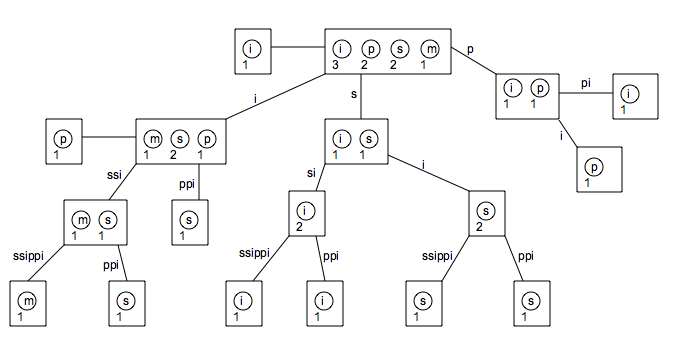
\includegraphics[width = 1\linewidth]{mississippi_suffix_tree.png}
  \caption{Suffix Tree with CRP Representation for "mississippi"}
  \label{fig:mississippiSuffixTree}
\end{figure}




\section{Prediction}
%input{Design}
%\chapter{Implementation}
\chapter{Testing}\label{chap:results}

\section{Perplexity}\label{sec:perplexity}

Language models are compared by evaluating the perplexity of the data for each. A better model has a smaller perplexity. Perplexity is defined in Equation \ref{eq:HD-perplexity}, where $H(Q;\hat{P})=\sum_{i}Q_{i}\log_{2}\hat{P_{i}}$ is the cross-entropy between the unknown true model $Q$ and the assumed model $\hat{P}$ \cite{mackay1995hierarchical}. For a bi-gram model, we can approximate this to Equation \ref{eq:HD-perplexity-approx}, where $T$ is the total number of words in the corpus.

\begin{equation}
\text{Perplexity}=2^{H(Q;\hat{P})}
\label{eq:HD-perplexity}
\end{equation}

\begin{equation}
\text{Perplexity}\simeq\left[\prod_{t=2}^{T}\hat{P}(w_{t}|w_{t-1})\right]^{-\frac{1}{T}}
\label{eq:HD-perplexity-approx}
\end{equation}

Another definition of perplexity is $2^{\ell(\boldsymbol{x})}$ where $\ell(\boldsymbol{x})$ is defined as in Equation \ref{eq:ellX} \cite{wood2011sequence}. This is relevant for the Sequence Memoizer implementation as it considers context of infinite length.

\begin{equation}
\ell(\boldsymbol{x})=-\frac{1}{|\boldsymbol{x}|}\sum_{i=1}^{|\boldsymbol{x}|}\log_{2}P(x_{i}|\boldsymbol{x}_{1:i-1})
\label{eq:ellX}
\end{equation}

Perplexity was found for the hierarchical Dirichlet model as in the following code. We find $P(i|j,D,\alpha\boldsymbol{m},\mathscr{H}_{D})$ for all bigrams as a vector, using the optimal values for $\alpha$ and $\boldsymbol{m}$. All elements in the vector are then multiplied together and the result is raised to the power $-\frac{1}{T}$, where $T$ is the total number of words in the corpus.



\section{Comparison of $n$-gram Smoothing Techniques}

\todo[inline]{Comparison of n-gram smoothing techniques}

\section{Evaluation of Hierarchical Models}

\todo[inline]{Evaluation of hierarchical models}

\section{Comparison of Model Performance with Wikipedia}

\todo[inline]{Comparison of model performance with wikipedia}

\chapter{Conclusion}
\bibliographystyle{unsrt}
\bibliography{Bibliography}
\end{document}